\chapter{Requirement Specifications} \label{chap:reqs}

%\version{v1.10.2015}

\section*{}
\section{Existing System vs Proposed System}

\begin{table}[h]
	\caption{\label{Related Systems} Comparisons.}
	\begin{tabular}{ |p{3cm}|p{6cm}|p{6cm}| }
		\hline
		\textbf{Application Name} & \textbf{Limitations}                                                                 & \textbf{Proposed Solution} \\
		\hline
		Zameen.com
		                          & No Project booking in app \newline No Payment through app
		                          & Project booking in app \newline No Payment through app \newline Track payment in app                              \\
		\hline
		Graana
		                          & No Project booking in app No \newline Payment through app
		                          & Project booking in app No \newline Payment through app \newline Track payment in app                              \\
		\hline
	\end{tabular}
\end{table}

\section{Functional CRM Requirements}
\subsection{CRO Customer Service}
CROs will be able to chat with customers through the Web Portal. Figure \ref{fig:crm_client}
\subsection{Client Customer Services}
Client will be able to contact the customer services of the projects they are affiliated with. They will do so by having a chatting interface. Figure \ref{fig:crm_agent}

\section{Functional Client Requirements [\nameref{client_view}]}
\subsection{Explore as Guest}
Clients will have availability to explore the application without registering to it. However, when they decide to make a booking, they will be prompted with a message to login first.
\subsection{Explore as Registered Account}
Clients will be able to Register and Login to the application to keep their data saved in the database. This will allow users to change their device without having to worry of losing their data.
\subsection{Edit Registered Account}
Clients will be able to change their profile's details through the application
\subsection{Book place in project}
Clients will be able to make booking in a project they desire. They will provide paid invoice in the start to authenticate their booking. Once authenticated by the admin, they will be shown in the application.
\subsection{Track Investments}
All the investments the client made will be shown in the app where they can track their payment records and make further payments.
\subsection{Schedule a Meeting}
Client will be able to schedule meetings with the owner through the app which will be approved by the admin through Web Portal
\subsection{Search}
Clients will be able to Search through the application with different filters and sorting options to best suit their needs and requirements.
\subsection{Add to Wish-list}
Clients will be able to add projects they like to their wish-list for later interest. Guests will have wish-lists stored on their device whereas logged in users will have it stored on the server.
\subsection{Add new Project}
Owners will be able to add new projects to their tally for clients to take interest in through the mobile app.
\subsection{View Scheduled Meetings}
Owners will be able to see the approved meetings by the admin on their phone and also reschedule  them if needed.
\subsection{Create Admin Account }
Owners will be able to create admin accounts for their managers.

\section{Functional ERP Requirements}
\subsection{Manage Meetings, Payments and Projects}
Managers who are given the admin credentials would be able to manage the projects, payments and meetings of their owner. Figure \ref{manage}
\subsection{Authenticate Payments}
Managers will be able to authenticate payments made by clients through web portal. Figure \ref{auth}
\subsection{Create CRO account}
Managers will be able to create new CRO accounts for customer services. Figure \ref{create}

\section{Functional Complaints Requirements}
\subsection{Register a complaint}
Clients will be able to register a complaint for the project they have invested in. Figure \ref{fig:cpm_register_user}
\subsection{Re send complaint}
Clients will be able to send a response to complaint for the project they have invested in. Figure \ref{fig:cpm_register_user}
\subsection{Reply to a complaint}
Admins will be able to reply to different complaints they receive. Figure Figure \ref{fig:cpm_admin}

\section{Non Functional Requirements}
\subsection{Encryption}
Passwords will be stored in encrypted form in the database. Other data that needs encryption such as payments will also be done so to keep proper security of the project.
\subsection{Performance}
Least amount of local storage will be used when data is fetched from the API. Only the required data such as tokens, wish lists, roles etc. will be stored. It will be noted that the API calls will be kept to minimum to avoid multiple API calls where a single one would be sufficient.
\subsection{Usability}
The User Interface would be kept extremely simple to understand and follow a color pattern to keep the user interaction simple. Things like submit buttons, back buttons will have a single component styling to help user memorize the functionality of each simply.

\newpage
\section{Use Cases}
\subsection{Diagrams}

% Your image goes here
\noindent
\begin{figure}[h]
	\makebox[\textwidth]{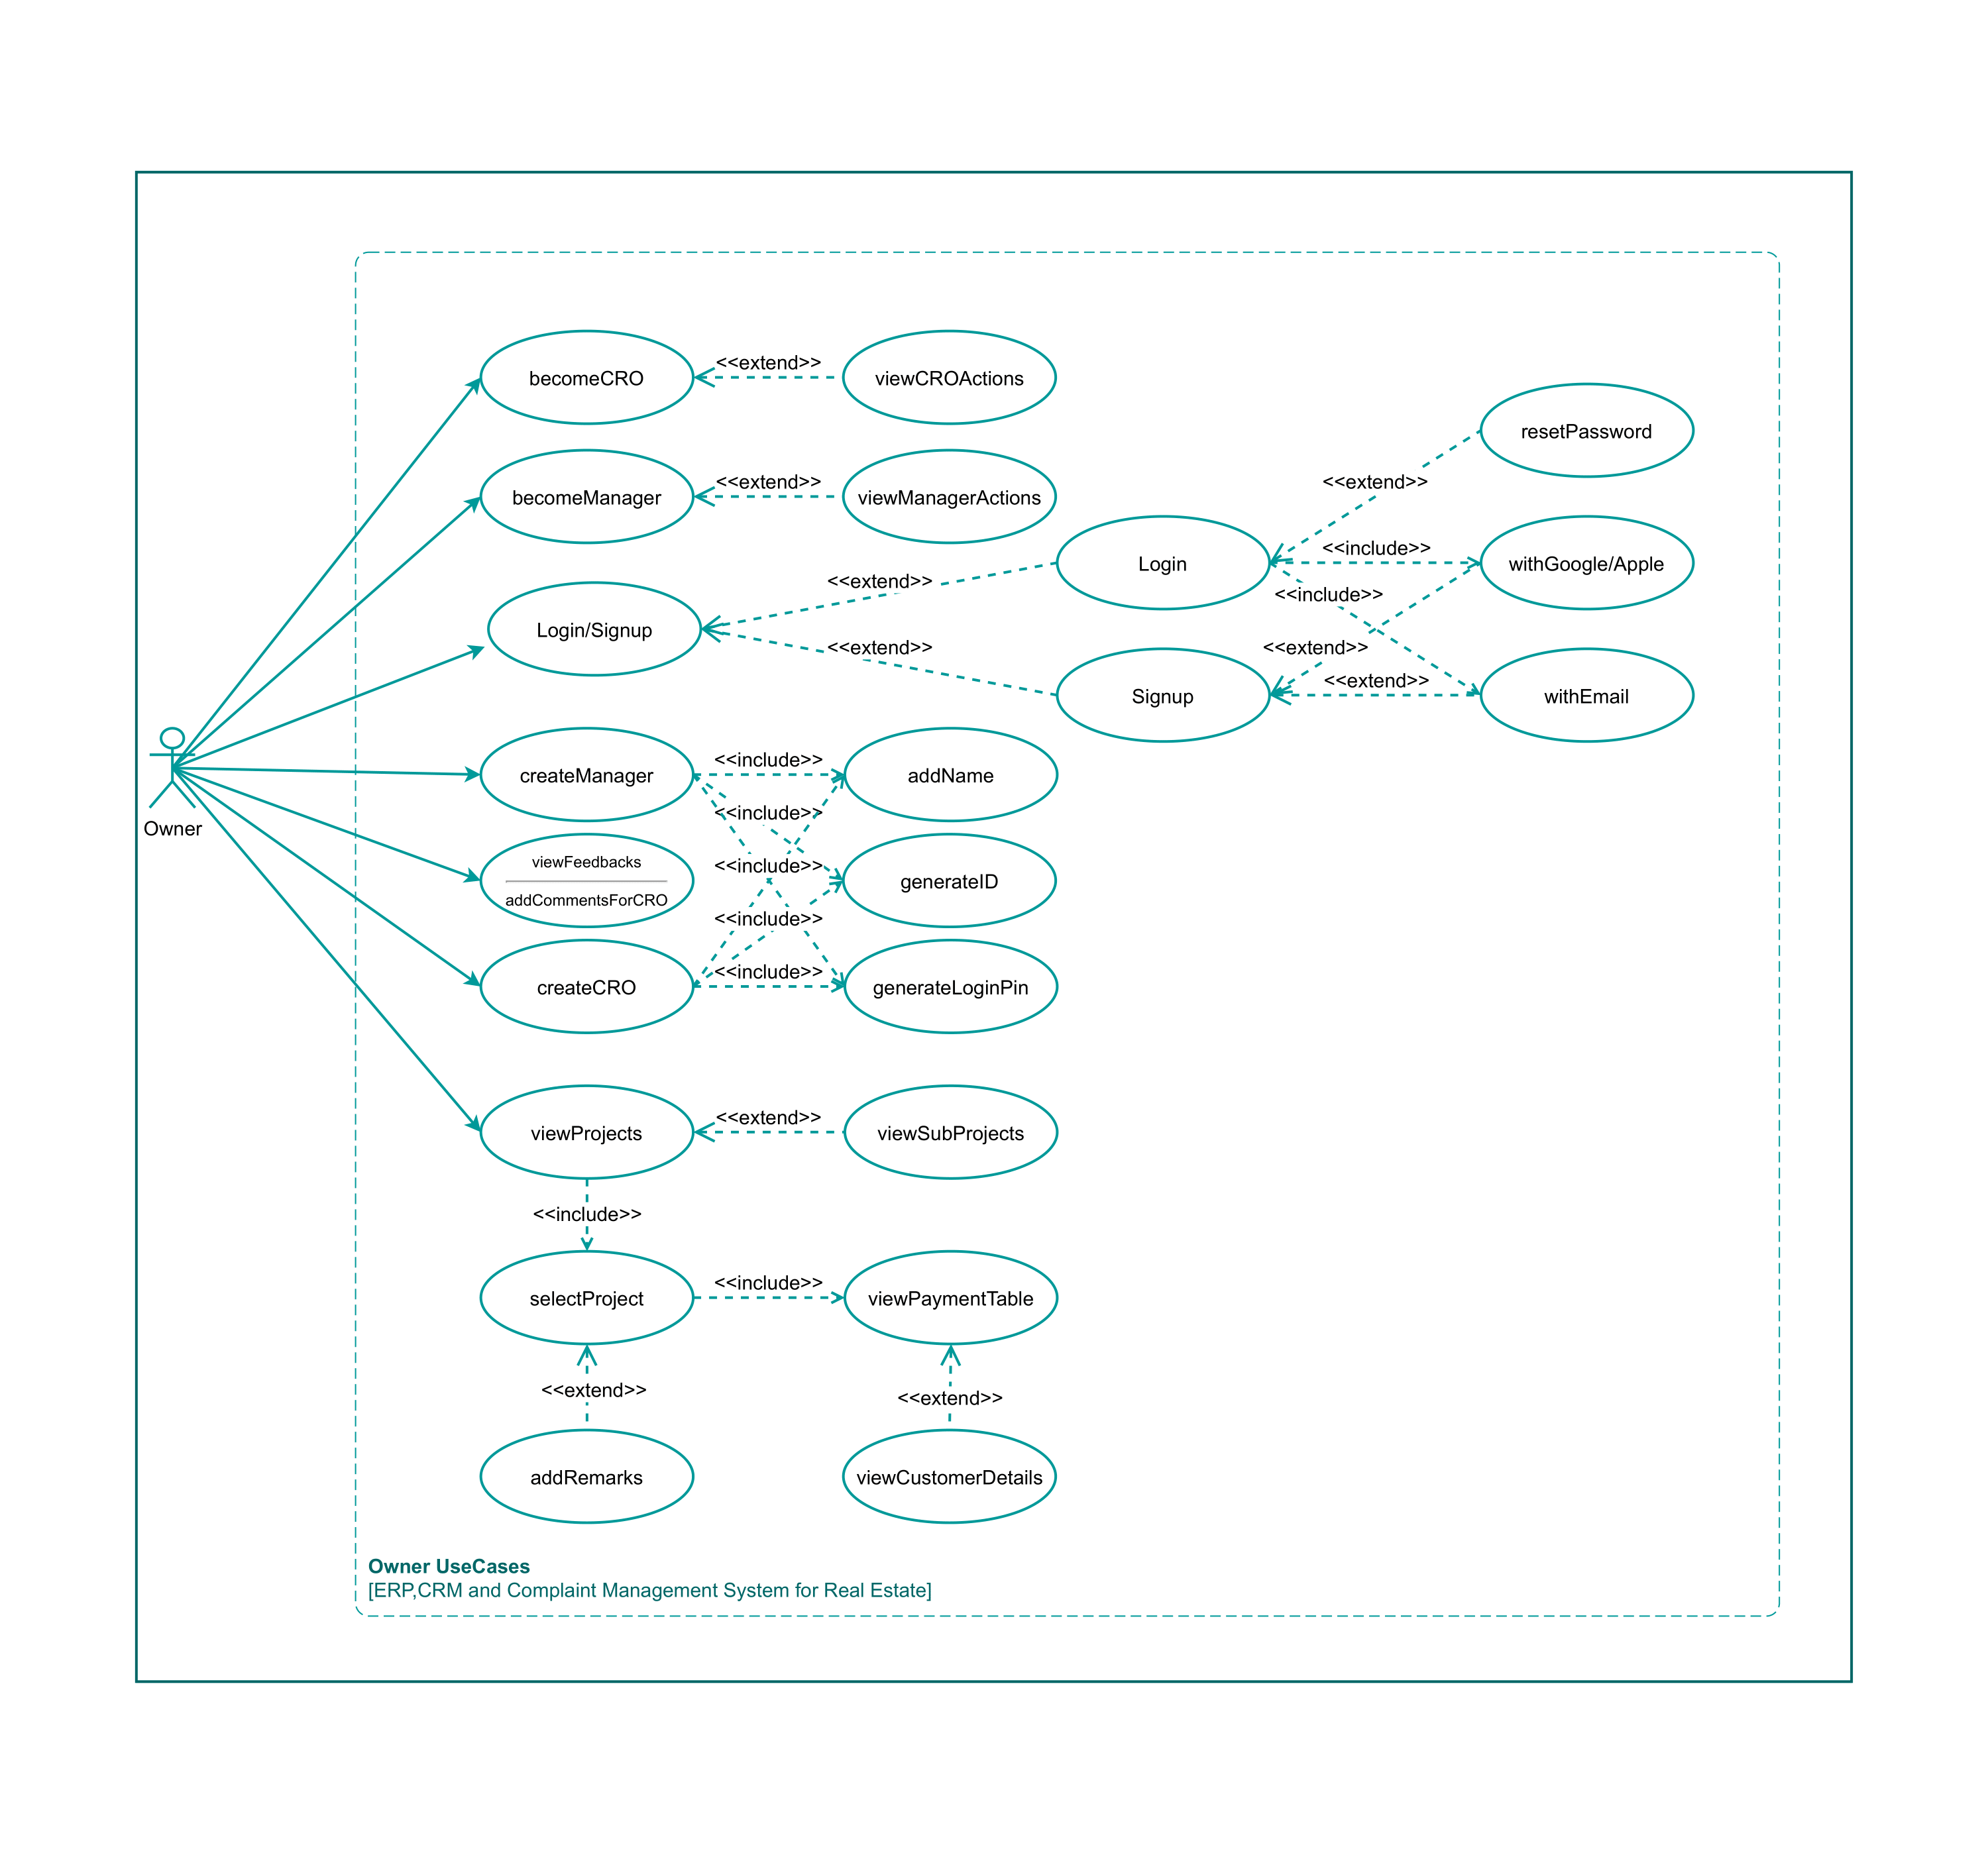
\includegraphics[scale=0.48]{figures/UseCase Diagrams/Use Case Diagram-1.png}}%
	\caption{Owner Use Case}
\end{figure}

\newpage
\begin{center}
	% Your image goes here

	\centerline{\noindent}%
	% \noindent
	\begin{figure}[h]
		\makebox[\textwidth]{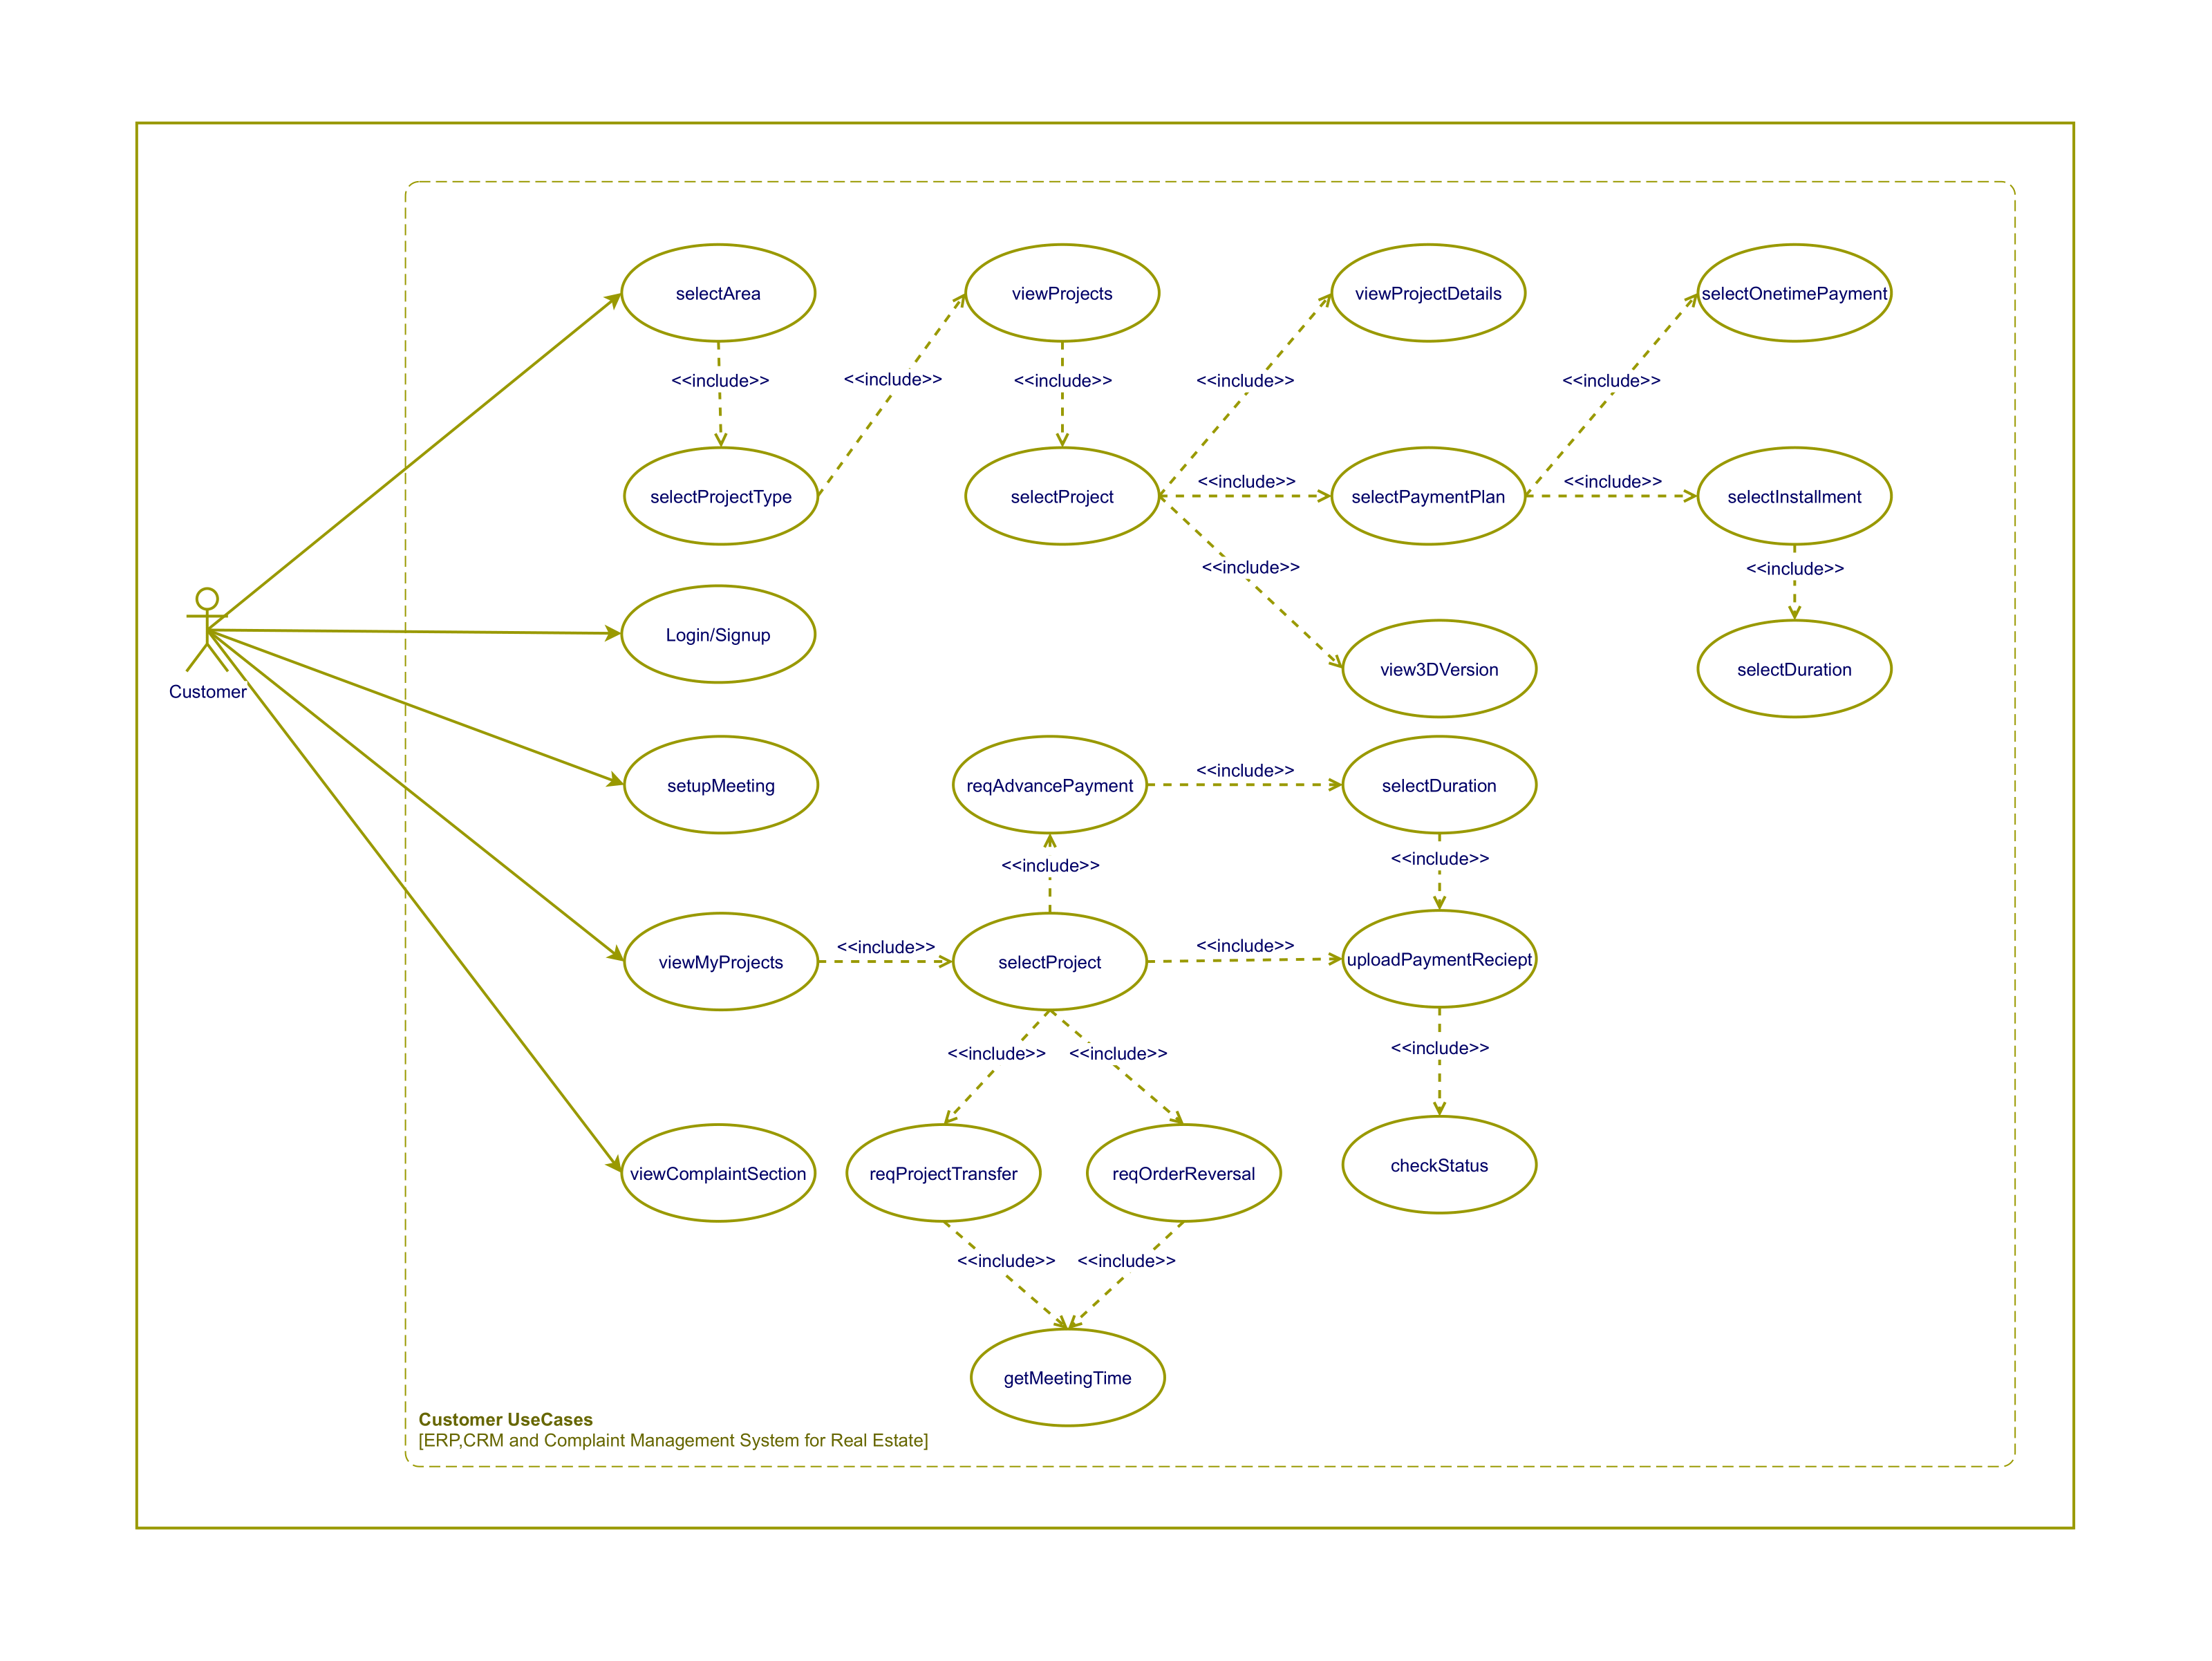
\includegraphics[scale=0.55]{figures/UseCase Diagrams/Use Case Diagram-3.png}}%
		\caption{Customer Use Case}
	\end{figure}

	% 
\end{center}


\newpage
\begin{center}
	% Your image goes here

	\centerline{\noindent}%
	% \noindent
	\begin{figure}[h]
		\makebox[\textwidth]{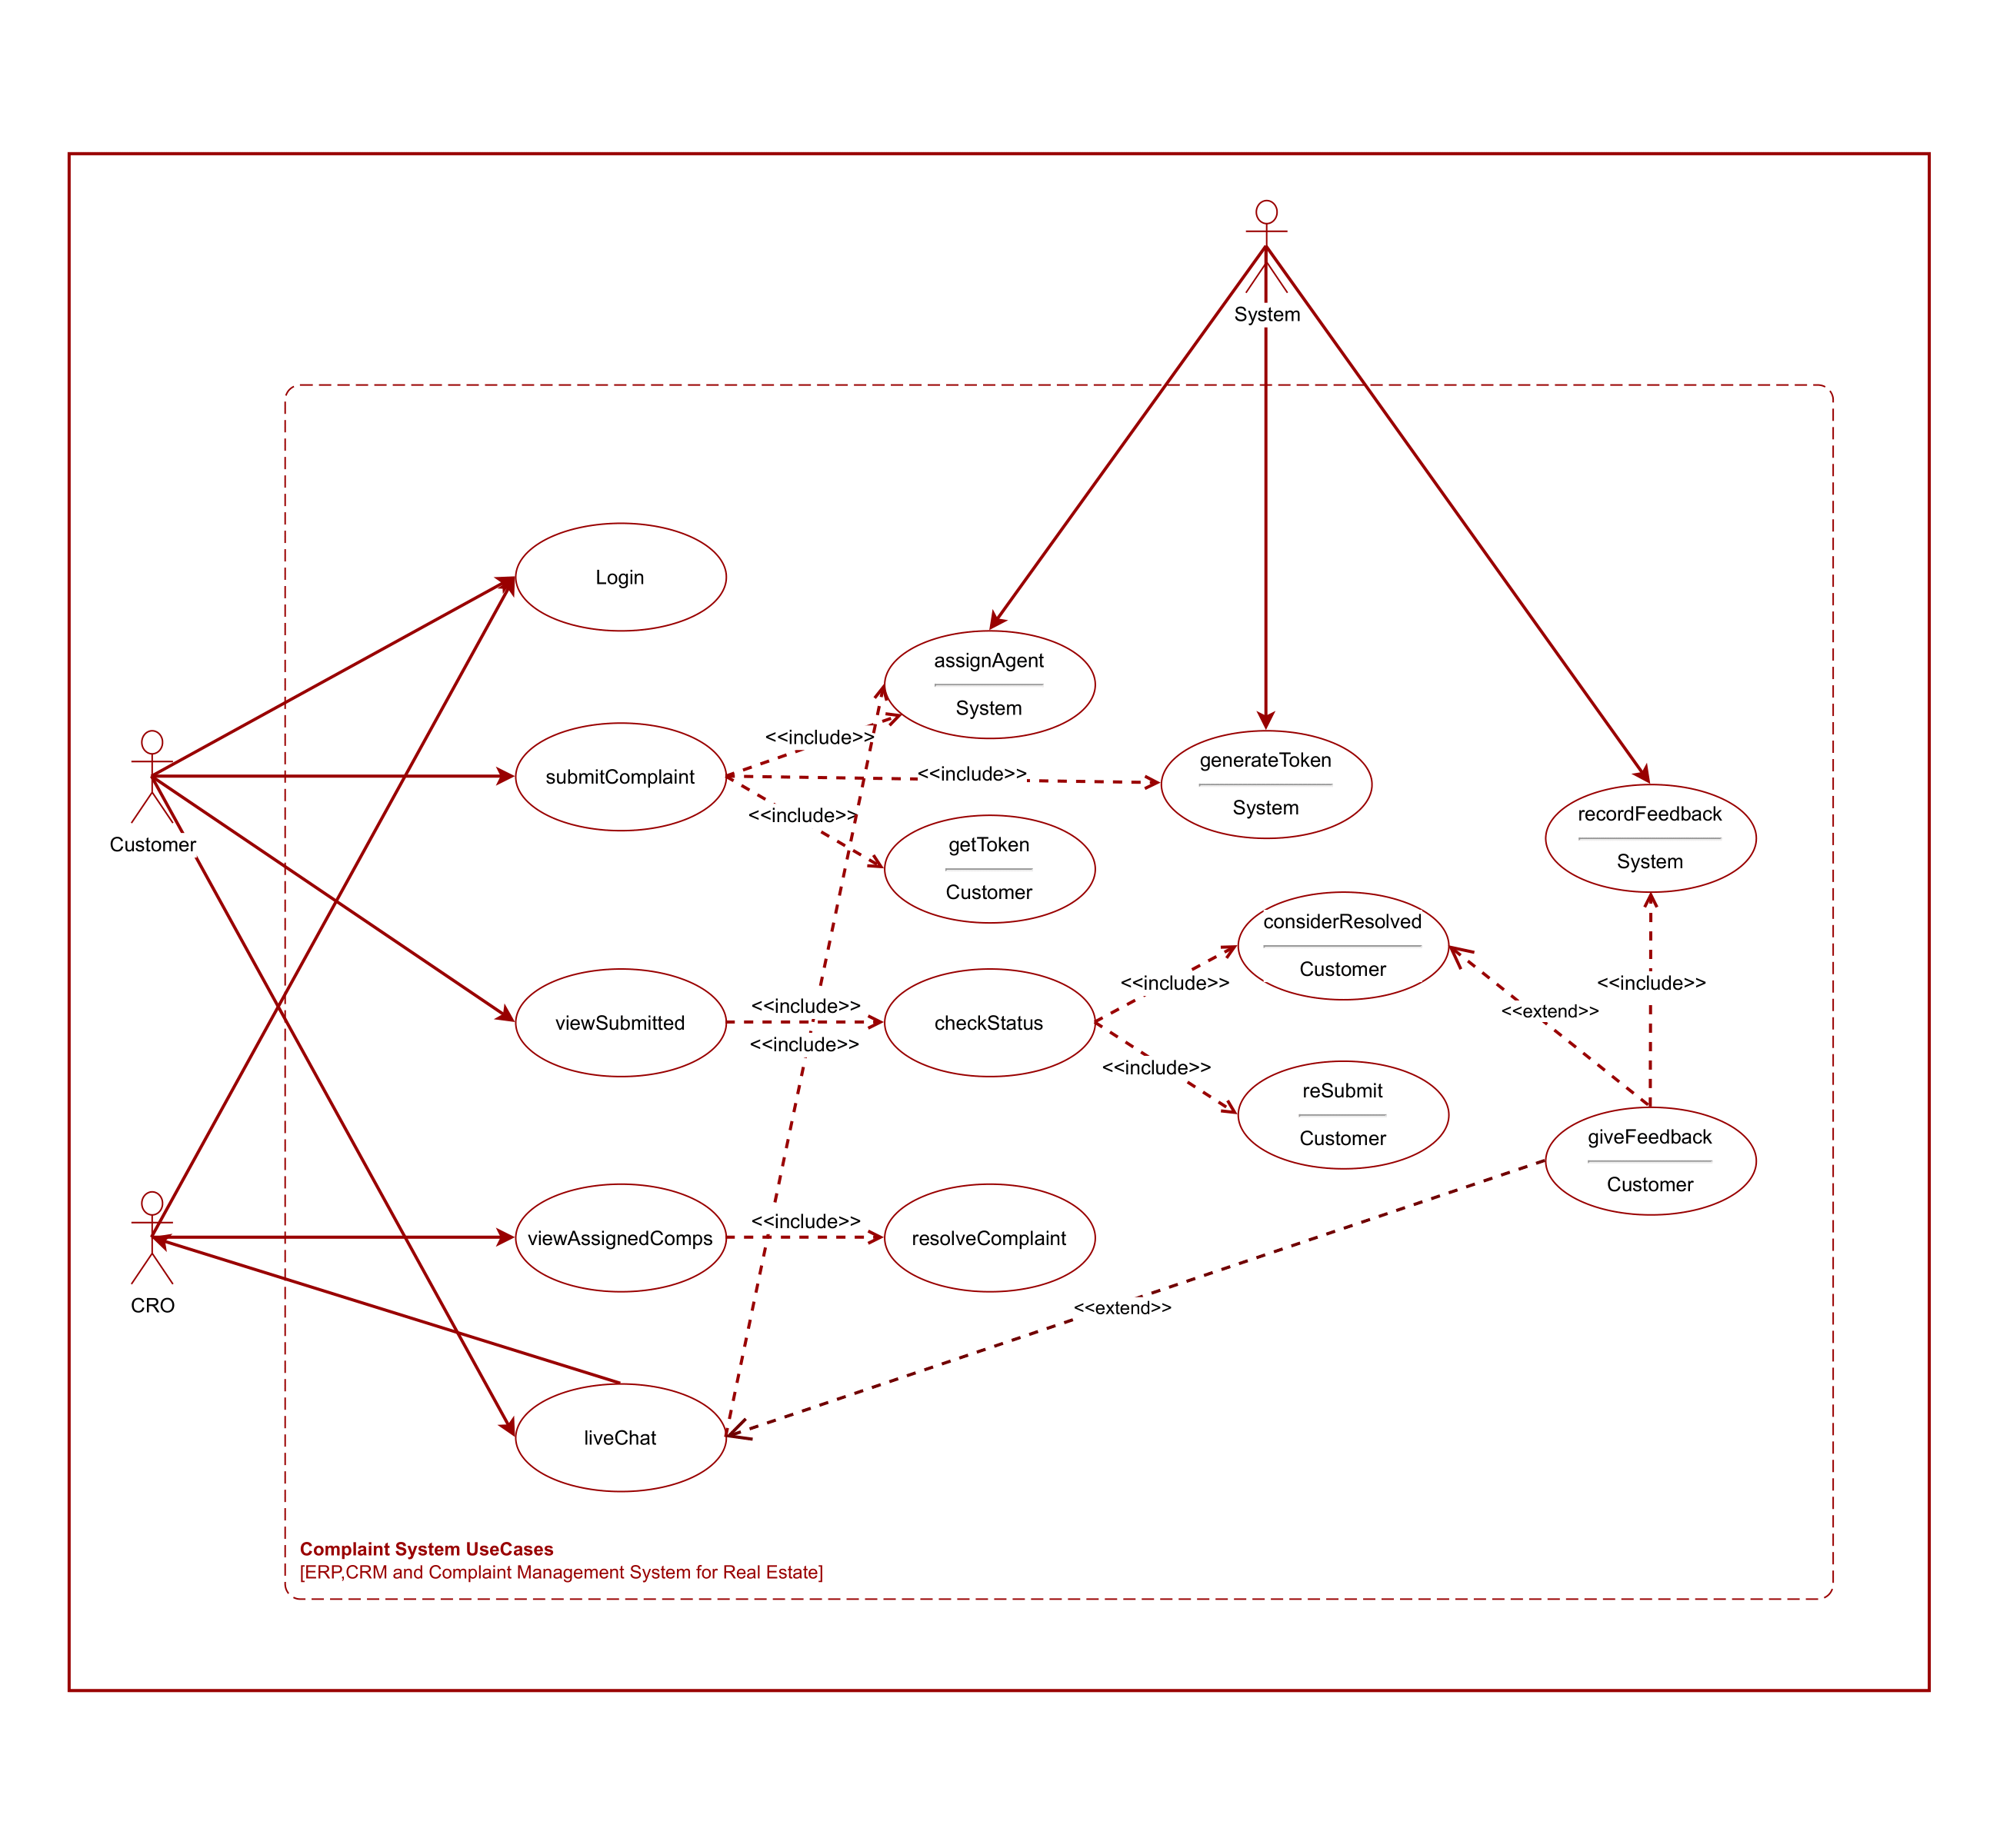
\includegraphics[scale=0.55]{figures/UseCase Diagrams/Use Case Diagram-4.png}}%
		\caption{CRO Use Case}
	\end{figure}

	% 
\end{center}


\newpage
\begin{center}
	% Your image goes here

	\centerline{\noindent}%
	% \noindent
	\begin{figure}[h]
		\makebox[\textwidth]{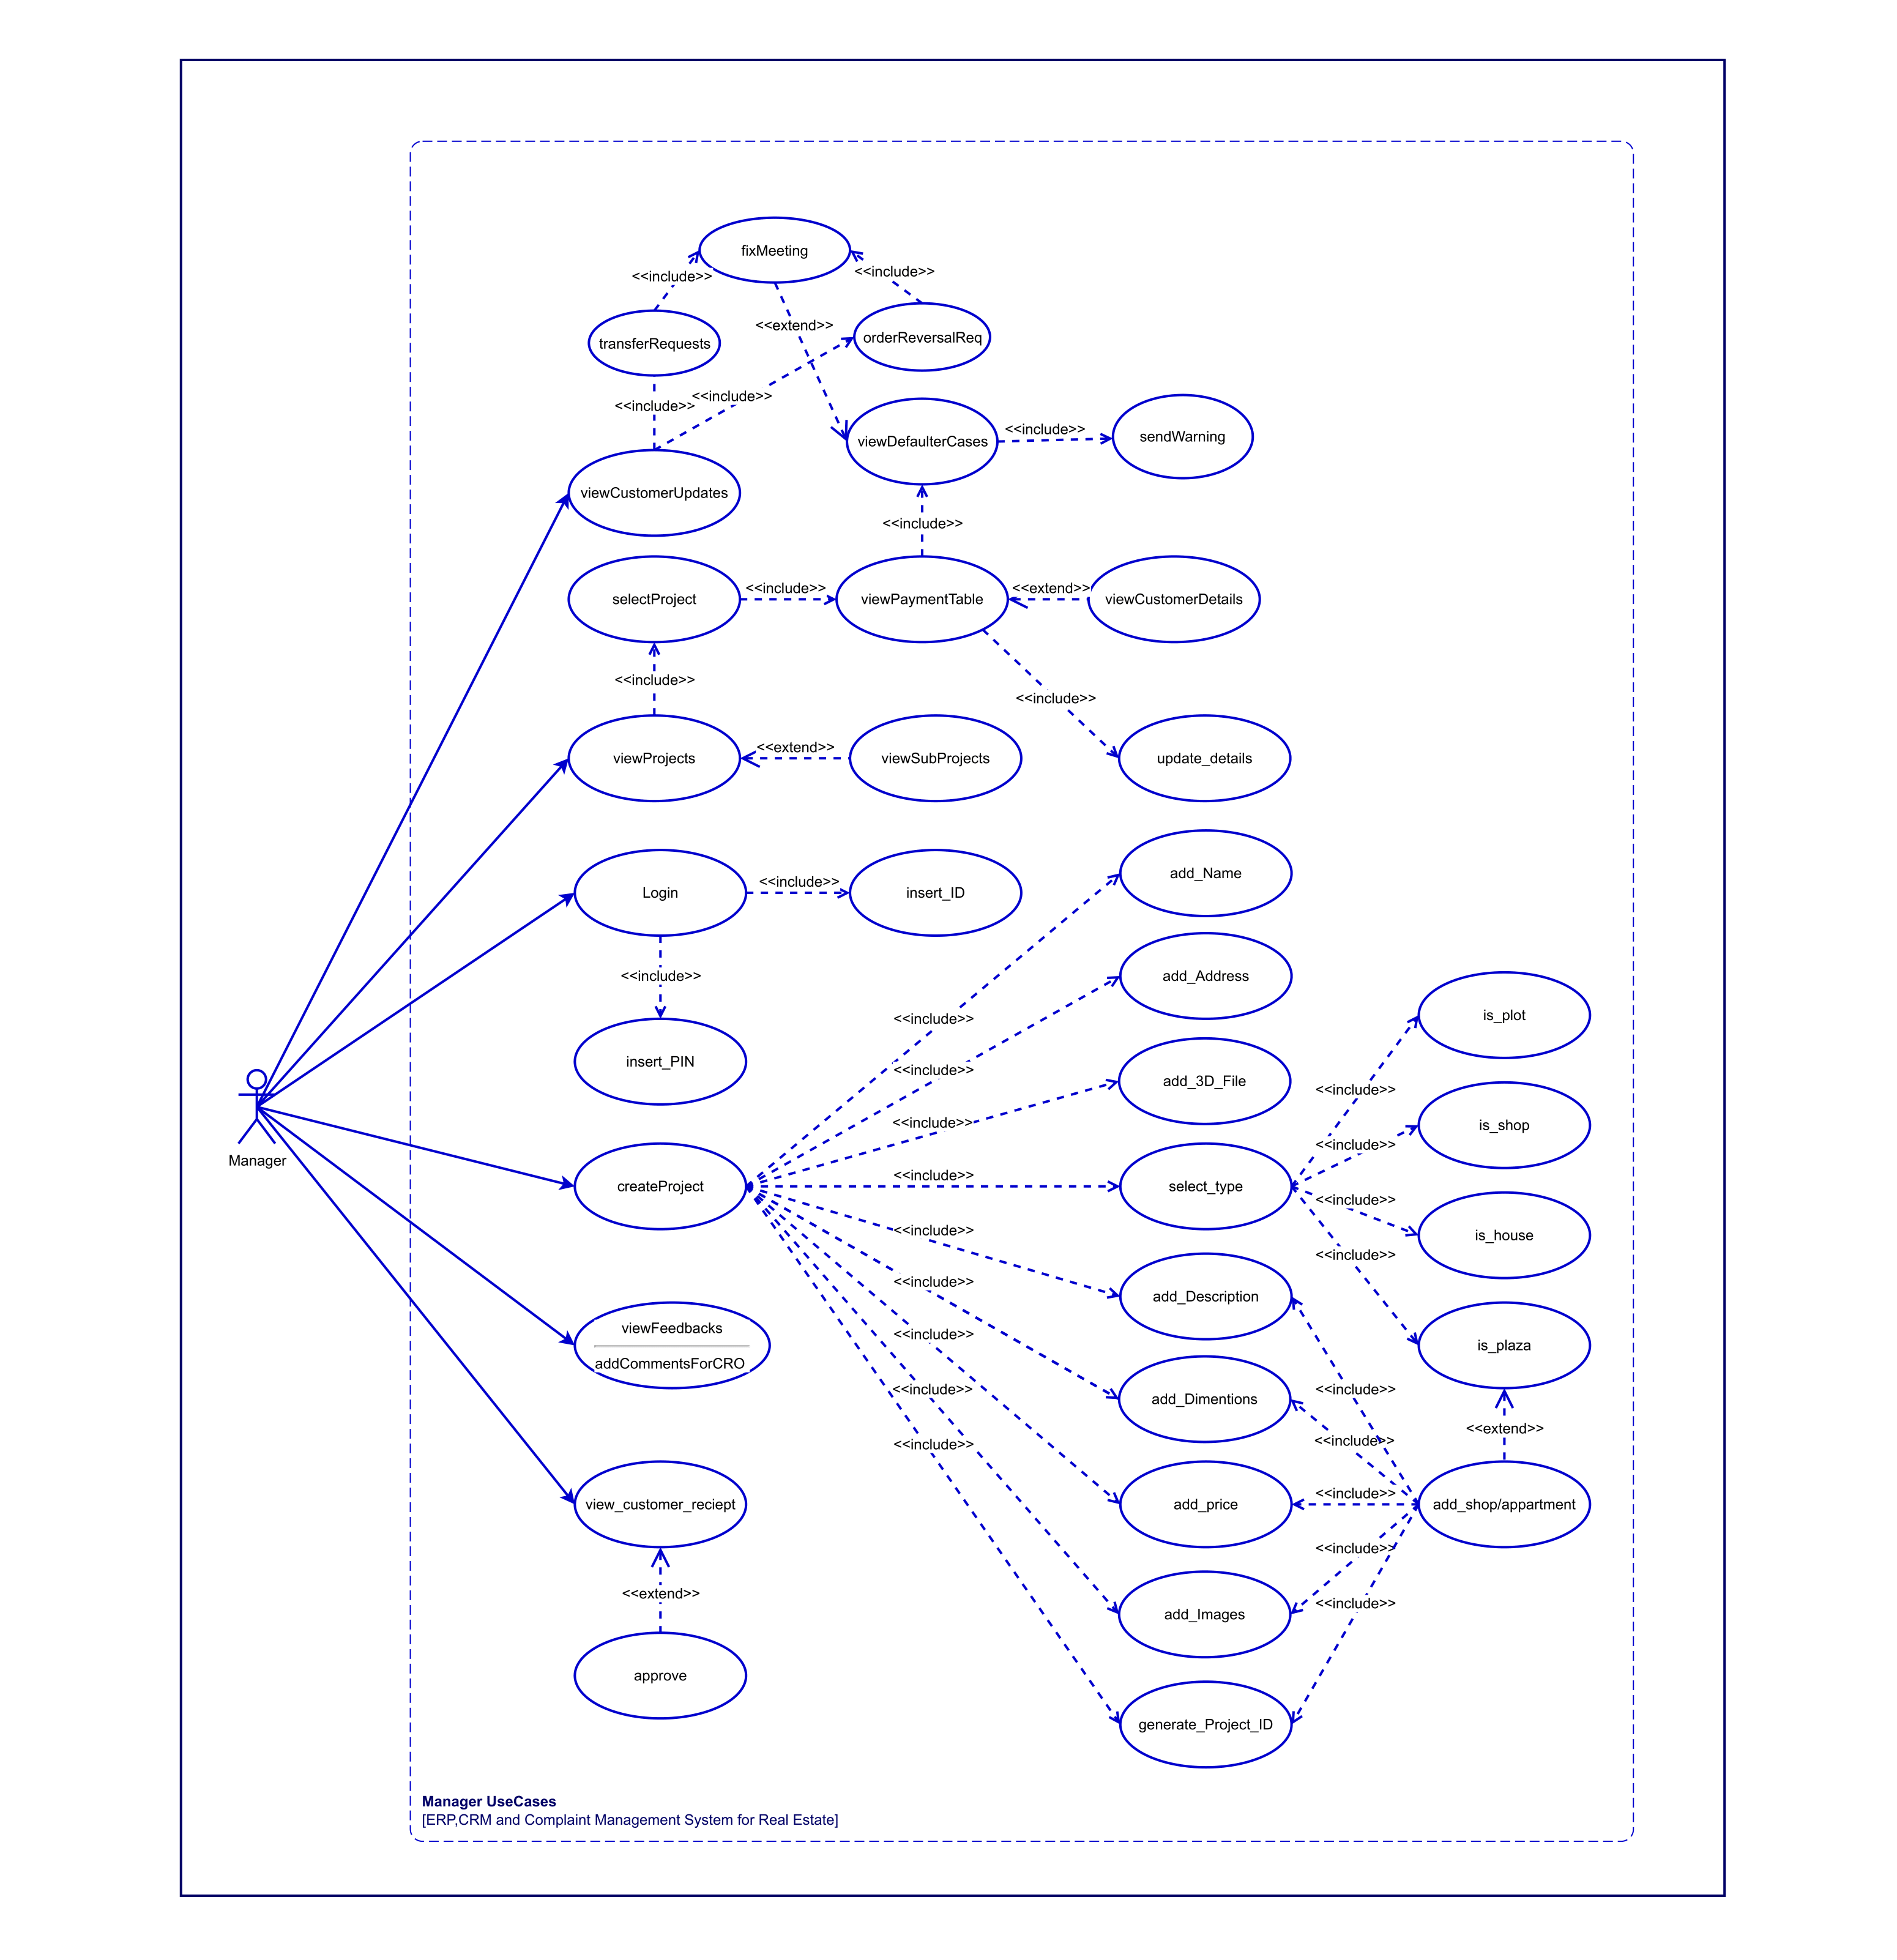
\includegraphics[scale=0.4]{figures/UseCase Diagrams/Use Case Diagram-2.png}}%
		\caption{Manager Use Case}
	\end{figure}

	% 
\end{center}
% \noindent
% \begin{figure}[h]
% 	\makebox[\textwidth]{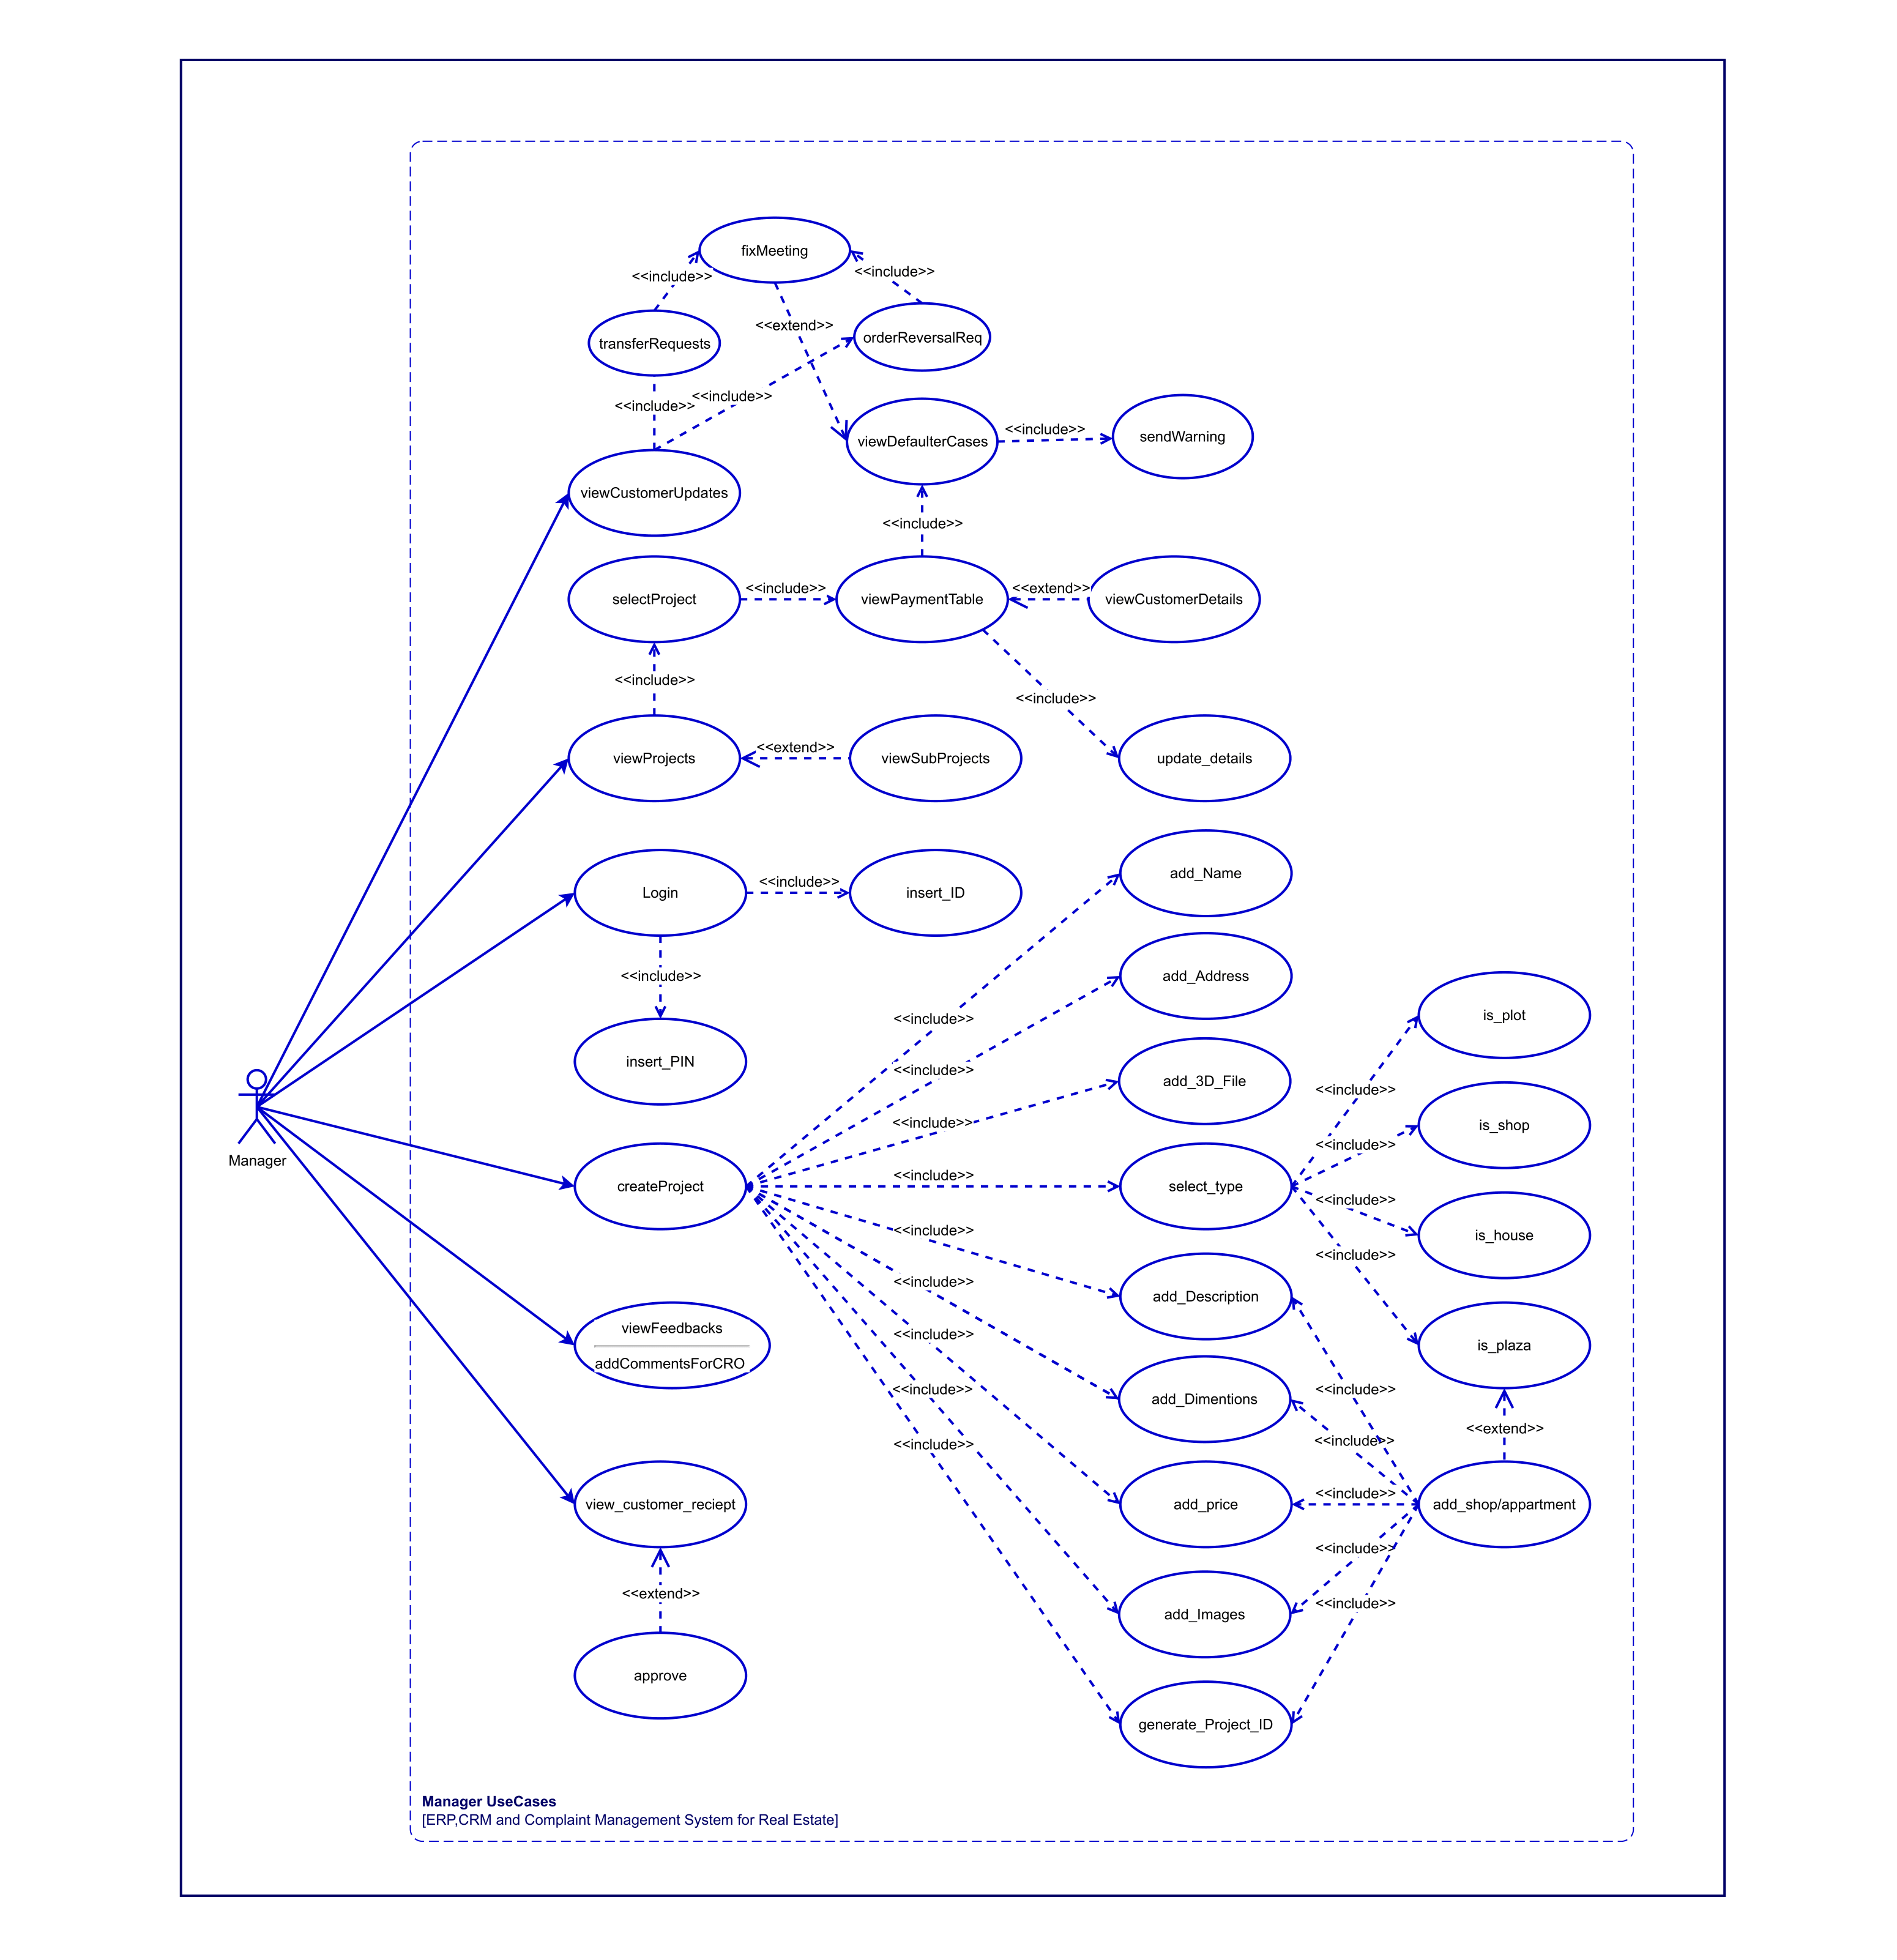
\includegraphics[scale=0.5]{figures/UseCase Diagrams/Use Case Diagram-2.png}}%
% \end{figure}

\newpage
\subsection{Description Tables}
% Please add the following required packages to your document preamble:
% \usepackage{multirow}
% \usepackage[table,xcdraw]{xcolor}
% If you use beamer only pass "xcolor=table" option, i.e. \documentclass[xcolor=table]{beamer}
\begin{table}[h]
    \caption{UC-001}
    \begin{tabular}{|l|p{5cm}p{5cm}|}
        \hline
        {\color[HTML]{231F20} \textbf{Use Case ID}}                                                     & \multicolumn{2}{l|}{{\color[HTML]{231F20} \textbf{UC-001}}}                                                                                                                                                                                                                                                                                                                                                                                                                                                                              \\ \hline
        \rowcolor[HTML]{CCCCCC}
        {\color[HTML]{231F20} \textbf{Use Case Name}}                                                   & \multicolumn{2}{l|}{\cellcolor[HTML]{CCCCCC}{\color[HTML]{231F20} Login}}                                                                                                                                                                                                                                                                                                                                                                                                                                                                \\ \hline
        {\color[HTML]{231F20} \textbf{Actors}}                                                          & \multicolumn{2}{l|}{{\color[HTML]{231F20} Owner,   Manager, Customer, CRO}}                                                                                                                                                                                                                                                                                                                                                                                                                                                              \\ \hline
        \rowcolor[HTML]{CCCCCC}
        {\color[HTML]{231F20} \textbf{Data}}                                                            & \multicolumn{2}{l|}{\cellcolor[HTML]{CCCCCC}{\color[HTML]{231F20} Username,   Password}}                                                                                                                                                                                                                                                                                                                                                                                                                                                 \\ \hline
        {\color[HTML]{231F20} \textbf{Trigger}}                                                         & \multicolumn{2}{l|}{{\color[HTML]{231F20} Press   on Login Button/Profile Tab}}                                                                                                                                                                                                                                                                                                                                                                                                                                                          \\ \hline
        \rowcolor[HTML]{CCCCCC}
        {\color[HTML]{231F20} \textbf{Pre-condition}}                                                   & \multicolumn{2}{l|}{\cellcolor[HTML]{CCCCCC}{\color[HTML]{231F20} Actor   should already have registered credentials.}}                                                                                                                                                                                                                                                                                                                                                                                                                  \\ \hline
        {\color[HTML]{231F20} \textbf{Assumptions}}                                                     & \multicolumn{2}{l|}{{\color[HTML]{231F20} Actors   have access to internet}}                                                                                                                                                                                                                                                                                                                                                                                                                                                             \\ \hline
        \rowcolor[HTML]{CCCCCC}
        \cellcolor[HTML]{CCCCCC}{\color[HTML]{231F20} }
                                                                                                        & \multicolumn{1}{c|}{\cellcolor[HTML]{CCCCCC}{\color[HTML]{231F20} \textbf{Actor Action}}}
                                                                                                        & \multicolumn{1}{c|}{\cellcolor[HTML]{CCCCCC}{\color[HTML]{231F20} \textbf{System Response}}}                                                                                                                                                                                                                                                                                                                                                                                                                                             \\ \cline{2-3}
        \rowcolor[HTML]{CCCCCC}
        \cellcolor[HTML]{CCCCCC}{\color[HTML]{231F20} }                                                 & \multicolumn{1}{l|}{\cellcolor[HTML]{CCCCCC}{\color[HTML]{231F20} }}                                                    & \cellcolor[HTML]{CCCCCC}{\color[HTML]{231F20} }                                                                                                                                                                                                                                                                                                                                                                \\
        \rowcolor[HTML]{CCCCCC}
        \cellcolor[HTML]{CCCCCC}{\color[HTML]{231F20} }                                                 & \multicolumn{1}{l|}{\multirow{-2}{*}{\cellcolor[HTML]{CCCCCC}{\color[HTML]{231F20} \textbf{Step 1:}}}}                  & \multirow{-2}{*}{\cellcolor[HTML]{CCCCCC}{\color[HTML]{231F20} \textbf{Step   2:}}}                                                                                                                                                                                                                                                                                                                            \\ \cline{2-3}
        \rowcolor[HTML]{CCCCCC}
        \multirow{-4}{*}{\cellcolor[HTML]{CCCCCC}{\color[HTML]{231F20} \textbf{Normal flow of events}}} & \multicolumn{1}{p{5cm}|}{\cellcolor[HTML]{CCCCCC}{\color[HTML]{231F20} Users   enter credentials in given fields}}      & {\color[HTML]{231F20} \begin{tabular}[c]{@{}p{5cm}@{}}If   the login is successful, they will\\      Have access to their profile. If the\\      Login is unsuccessful, they will be \\      Prompted with a message to try again \\      Or signup for account.\\      In case of Manager and CRO, they\\      Will be told to ask their Owner/Manager to provide them\\      with credentials.\end{tabular}} \\ \hline
        {\color[HTML]{231F20} }                                                                         & \multicolumn{2}{l|}{{\color[HTML]{231F20} ·         Login Fails}}                                                                                                                                                                                                                                                                                                                                                                                                                                                                        \\ \cline{2-3}
        \multirow{-2}{*}{{\color[HTML]{231F20} \textbf{Alternate flow of events}}}                      & \multicolumn{2}{l|}{{\color[HTML]{231F20} ·       Prompted   with message}}                                                                                                                                                                                                                                                                                                                                                                                                                                                              \\ \hline
        \rowcolor[HTML]{CCCCCC}
        {\color[HTML]{231F20} \textbf{Main success scenarios}}                                          & \multicolumn{2}{l|}{\cellcolor[HTML]{CCCCCC}{\color[HTML]{231F20} Login   succeeds}}                                                                                                                                                                                                                                                                                                                                                                                                                                                     \\ \hline
        {\color[HTML]{231F20} \textbf{Post-condition}}                                                  & \multicolumn{2}{l|}{{\color[HTML]{231F20} User   gets access to their profile.}}                                                                                                                                                                                                                                                                                                                                                                                                                                                         \\ \hline
    \end{tabular}
\end{table}
% Please add the following required packages to your document preamble:
% \usepackage{multirow}
% \usepackage[table,xcdraw]{xcolor}
% If you use beamer only pass "xcolor=table" option, i.e. \documentclass[xcolor=table]{beamer}
\begin{table}[h]
    \caption{UC-002}
    \begin{tabular}{|l|p{5cm}p{5cm}|}
        \hline
        {\color[HTML]{231F20} \textbf{Use Case ID}}                                                      & \multicolumn{2}{l|}{{\color[HTML]{231F20} \textbf{UC-002}}}                                                                                                                                                                                                               \\ \hline
        \rowcolor[HTML]{CCCCCC}
        {\color[HTML]{231F20} \textbf{Use Case Name}}                                                    & \multicolumn{2}{l|}{\cellcolor[HTML]{CCCCCC}{\color[HTML]{231F20} Sign   up}}                                                                                                                                                                                             \\ \hline
        {\color[HTML]{231F20} \textbf{Actors}}                                                           & \multicolumn{2}{l|}{{\color[HTML]{231F20} Owner,   Customer}}                                                                                                                                                                                                             \\ \hline
        \rowcolor[HTML]{CCCCCC}
        {\color[HTML]{231F20} \textbf{Data}}                                                             & \multicolumn{2}{l|}{\cellcolor[HTML]{CCCCCC}{\color[HTML]{231F20} Email   or Google/Apple ID.}}                                                                                                                                                                           \\ \hline
        {\color[HTML]{231F20} \textbf{Trigger}}                                                          & \multicolumn{2}{l|}{{\color[HTML]{231F20} Press   on Sign Up Button}}                                                                                                                                                                                                     \\ \hline
        \rowcolor[HTML]{CCCCCC}
        {\color[HTML]{231F20} \textbf{Pre-condition}}                                                    & \multicolumn{2}{l|}{\cellcolor[HTML]{CCCCCC}{\color[HTML]{231F20} Have   access to Application}}                                                                                                                                                                          \\ \hline
        {\color[HTML]{231F20} \textbf{Assumptions}}                                                      & \multicolumn{2}{l|}{{\color[HTML]{231F20} Actors   have access to internet}}                                                                                                                                                                                              \\ \hline
        \rowcolor[HTML]{CCCCCC}
        \cellcolor[HTML]{CCCCCC}{\color[HTML]{231F20} }
                                                                                                         & \multicolumn{1}{c|}{\cellcolor[HTML]{CCCCCC}{\color[HTML]{231F20} \textbf{Actor Action}}}
                                                                                                         & \multicolumn{1}{c|}{\cellcolor[HTML]{CCCCCC}{\color[HTML]{231F20} \textbf{System Response}}}                                                                                                                                                                              \\ \cline{2-3}
        \rowcolor[HTML]{CCCCCC}
        \cellcolor[HTML]{CCCCCC}{\color[HTML]{231F20} }                                                  & \multicolumn{1}{l|}{\cellcolor[HTML]{CCCCCC}{\color[HTML]{231F20} }}                                                                             & \cellcolor[HTML]{CCCCCC}{\color[HTML]{231F20} }                                                                        \\
        \rowcolor[HTML]{CCCCCC}
        \cellcolor[HTML]{CCCCCC}{\color[HTML]{231F20} }                                                  & \multicolumn{1}{l|}{\multirow{-2}{*}{\cellcolor[HTML]{CCCCCC}{\color[HTML]{231F20} \textbf{Step 1:}}}}                                           & \multirow{-2}{*}{\cellcolor[HTML]{CCCCCC}{\color[HTML]{231F20} \textbf{Step   2:}}}                                    \\ \cline{2-3}
        \rowcolor[HTML]{CCCCCC}
        \cellcolor[HTML]{CCCCCC}{\color[HTML]{231F20} }                                                  & \multicolumn{1}{p{5cm}|}{\cellcolor[HTML]{CCCCCC}{\color[HTML]{231F20} Actor can use their Google/Apple   ID to create account.}}                & {\color[HTML]{231F20} If same email or invalid email is being used   for sign-up, user will be prompted to change it.} \\ \cline{2-3}
        \rowcolor[HTML]{CCCCCC}
        \cellcolor[HTML]{CCCCCC}{\color[HTML]{231F20} }                                                  & \multicolumn{1}{p{5cm}|}{\cellcolor[HTML]{CCCCCC}{\color[HTML]{231F20} They will have majority of the   fields of sign-up form already filled.}} & {\color[HTML]{231F20} If the sign-up completes, they can use their   account to login.}                                \\ \cline{2-3}
        \rowcolor[HTML]{CCCCCC}
        \cellcolor[HTML]{CCCCCC}{\color[HTML]{231F20} }                                                  & \multicolumn{1}{p{5cm}|}{\cellcolor[HTML]{CCCCCC}{\color[HTML]{231F20} Actor can also use their email to   create account.}}                     & {\color[HTML]{231F20} On failure of sign-up, they get prompted with   respective reasons}                              \\ \cline{2-3}
        \rowcolor[HTML]{CCCCCC}
        \multirow{-25}{*}{\cellcolor[HTML]{CCCCCC}{\color[HTML]{231F20} \textbf{Normal flow of events}}} & \multicolumn{1}{p{5cm}|}{\cellcolor[HTML]{CCCCCC}{\color[HTML]{231F20} They would provide details in   required fields of sign-up columns.}}     &                                                                                                                        \\ \hline
        {\color[HTML]{231F20} }                                                                          & \multicolumn{2}{l|}{{\color[HTML]{231F20} ·         Signup Fails}}                                                                                                                                                                                                        \\ \cline{2-3}
        \multirow{-2}{*}{{\color[HTML]{231F20} \textbf{Alternate flow of events}}}                       & \multicolumn{2}{l|}{{\color[HTML]{231F20} ·       Prompted   with message}}                                                                                                                                                                                               \\ \hline
        \rowcolor[HTML]{CCCCCC}
        {\color[HTML]{231F20} \textbf{Main success scenarios}}                                           & \multicolumn{2}{l|}{\cellcolor[HTML]{CCCCCC}{\color[HTML]{231F20} Signup   succeeds and mail is sent to user for authentication.}}                                                                                                                                        \\ \hline
        {\color[HTML]{231F20} \textbf{Post-condition}}                                                   & \multicolumn{2}{l|}{{\color[HTML]{231F20} Actor   can login using the credentials provided during signup}}                                                                                                                                                                \\ \hline
    \end{tabular}
\end{table}
% Please add the following required packages to your document preamble:
% \usepackage{multirow}
% \usepackage[table,xcdraw]{xcolor}
% If you use beamer only pass "xcolor=table" option, i.e. \documentclass[xcolor=table]{beamer}
\begin{table}[]
    \caption{UC-003}
    \begin{tabular}{|l|p{5cm}p{5cm}|}
        \hline
        {\color[HTML]{231F20} \textbf{Use Case ID}}                                                      & \multicolumn{2}{l|}{{\color[HTML]{231F20} \textbf{UC-003}}}                                                                                                                                                                                                   \\ \hline
        \rowcolor[HTML]{CCCCCC}
        {\color[HTML]{231F20} \textbf{Use Case Name}}                                                    & \multicolumn{2}{l|}{\cellcolor[HTML]{CCCCCC}{\color[HTML]{231F20} Reset Password}}                                                                                                                                                                            \\ \hline
        {\color[HTML]{231F20} \textbf{Actors}}                                                           & \multicolumn{2}{l|}{{\color[HTML]{231F20} Owner, Customer}}                                                                                                                                                                                                   \\ \hline
        \rowcolor[HTML]{CCCCCC}
        {\color[HTML]{231F20} \textbf{Data}}                                                             & \multicolumn{2}{l|}{\cellcolor[HTML]{CCCCCC}{\color[HTML]{231F20} Email/Username associated with   account}}                                                                                                                                                  \\ \hline
        {\color[HTML]{231F20} \textbf{Trigger}}                                                          & \multicolumn{2}{l|}{{\color[HTML]{231F20} Select Forgot Password button}}                                                                                                                                                                                     \\ \hline
        \rowcolor[HTML]{CCCCCC}
        {\color[HTML]{231F20} \textbf{Pre-condition}}                                                    & \multicolumn{2}{l|}{\cellcolor[HTML]{CCCCCC}{\color[HTML]{231F20} Have access to application}}                                                                                                                                                                \\ \hline
        {\color[HTML]{231F20} \textbf{Assumptions}}                                                      & \multicolumn{2}{l|}{{\color[HTML]{231F20} Actors have access to internet}}                                                                                                                                                                                    \\ \hline
        \rowcolor[HTML]{CCCCCC}
        \cellcolor[HTML]{CCCCCC}{\color[HTML]{231F20} }
                                                                                                         & \multicolumn{1}{c|}{\cellcolor[HTML]{CCCCCC}{\color[HTML]{231F20} \textbf{Actor Action}}}
                                                                                                         & \multicolumn{1}{c|}{\cellcolor[HTML]{CCCCCC}{\color[HTML]{231F20} \textbf{System Response}}}                                                                                                                                                                  \\ \cline{2-3}
        \rowcolor[HTML]{CCCCCC}
        \cellcolor[HTML]{CCCCCC}{\color[HTML]{231F20} }                                                  & \multicolumn{1}{p{5cm}|}{\cellcolor[HTML]{CCCCCC}{\color[HTML]{231F20} }}                                                                    & \cellcolor[HTML]{CCCCCC}{\color[HTML]{231F20} }                                                                \\
        \rowcolor[HTML]{CCCCCC}
        \cellcolor[HTML]{CCCCCC}{\color[HTML]{231F20} }                                                  & \multicolumn{1}{p{5cm}|}{\multirow{-2}{*}{\cellcolor[HTML]{CCCCCC}{\color[HTML]{231F20} \textbf{Step 1:}}}}                                  & \multirow{-2}{*}{\cellcolor[HTML]{CCCCCC}{\color[HTML]{231F20} \textbf{Step 2:}}}                              \\ \cline{2-3}
        \rowcolor[HTML]{CCCCCC}
        \cellcolor[HTML]{CCCCCC}{\color[HTML]{231F20} }                                                  & \multicolumn{1}{p{5cm}|}{\cellcolor[HTML]{CCCCCC}{\color[HTML]{231F20} User will provide their username/email associated with the account.}} & \cellcolor[HTML]{CCCCCC}{\color[HTML]{231F20} }                                                                \\ \cline{2-2}
        \rowcolor[HTML]{CCCCCC}
        \cellcolor[HTML]{CCCCCC}{\color[HTML]{231F20} }                                                  & \multicolumn{1}{p{5cm}|}{\cellcolor[HTML]{CCCCCC}{\color[HTML]{231F20} They will be mailed a link which will reset their password.}}         & \cellcolor[HTML]{CCCCCC}{\color[HTML]{231F20} }                                                                \\ \cline{2-2}
        \rowcolor[HTML]{CCCCCC}
        \cellcolor[HTML]{CCCCCC}{\color[HTML]{231F20} }                                                  & \multicolumn{1}{p{5cm}|}{\cellcolor[HTML]{CCCCCC}{\color[HTML]{231F20} On that link, they will be able to provide new password.}}            & \cellcolor[HTML]{CCCCCC}{\color[HTML]{231F20} }                                                                \\ \cline{2-2}
        \rowcolor[HTML]{CCCCCC}
        \multirow{-25}{*}{\cellcolor[HTML]{CCCCCC}{\color[HTML]{231F20} \textbf{Normal flow of events}}} & \multicolumn{1}{p{5cm}|}{\cellcolor[HTML]{CCCCCC}{\color[HTML]{231F20} The link will expire after 5 minutes}}                                & \multirow{-17}{=}{\cellcolor[HTML]{CCCCCC}{\color[HTML]{231F20} User will be prompted to check   their mail.}} \\ \hline
        {\color[HTML]{231F20} }                                                                          & \multicolumn{2}{l|}{{\color[HTML]{231F20} ·       Site   is down}}                                                                                                                                                                                            \\ \cline{2-3}
        \multirow{-2}{*}{{\color[HTML]{231F20} \textbf{Alternate flow of   events}}}                     & \multicolumn{2}{l|}{{\color[HTML]{231F20} ·       No email is sent}}                                                                                                                                                                                          \\ \hline
        \rowcolor[HTML]{CCCCCC}
        {\color[HTML]{231F20} \textbf{Main success scenarios}}                                           & \multicolumn{2}{l|}{\cellcolor[HTML]{CCCCCC}{\color[HTML]{231F20} Resetting of Password Succeeds.}}                                                                                                                                                           \\ \hline
        {\color[HTML]{231F20} \textbf{Post-condition}}                                                   & \multicolumn{2}{l|}{{\color[HTML]{231F20} User can use new password to login   to their account}}                                                                                                                                                             \\ \hline
    \end{tabular}
\end{table}
% Please add the following required packages to your document preamble:
% \usepackage{multirow}
% \usepackage[table,xcdraw]{xcolor}
% If you use beamer only pass "xcolor=table" option, i.e. \documentclass[xcolor=table]{beamer}
\begin{table}[h]
    \caption{UC-004}
    \begin{tabular}{|l|p{5cm}p{5cm}|}
        \hline
        {\color[HTML]{231F20} \textbf{Use Case ID}}                                                     & \multicolumn{2}{l|}{{\color[HTML]{231F20} \textbf{UC-004}}}                                                                                                                                                                                                       \\ \hline
        \rowcolor[HTML]{CCCCCC}
        {\color[HTML]{231F20} \textbf{Use Case Name}}                                                   & \multicolumn{2}{l|}{\cellcolor[HTML]{CCCCCC}{\color[HTML]{231F20} Create   a Manager Account}}                                                                                                                                                                    \\ \hline
        {\color[HTML]{231F20} \textbf{Actors}}                                                          & \multicolumn{2}{l|}{{\color[HTML]{231F20} Owner}}                                                                                                                                                                                                                 \\ \hline
        \rowcolor[HTML]{CCCCCC}
        {\color[HTML]{231F20} \textbf{Data}}                                                            & \multicolumn{2}{l|}{\cellcolor[HTML]{CCCCCC}{\color[HTML]{231F20} Manager’s   email and other details.}}                                                                                                                                                          \\ \hline
        {\color[HTML]{231F20} \textbf{Trigger}}                                                         & \multicolumn{2}{l|}{{\color[HTML]{231F20} Click   on add a manager button}}                                                                                                                                                                                       \\ \hline
        \rowcolor[HTML]{CCCCCC}
        {\color[HTML]{231F20} \textbf{Pre-condition}}                                                   & \multicolumn{2}{l|}{\cellcolor[HTML]{CCCCCC}{\color[HTML]{231F20} Already   logged in}}                                                                                                                                                                           \\ \hline
        {\color[HTML]{231F20} \textbf{Assumptions}}                                                     & \multicolumn{2}{l|}{{\color[HTML]{231F20} Actors   have access to internet}}                                                                                                                                                                                      \\ \hline
        \rowcolor[HTML]{CCCCCC}
        \cellcolor[HTML]{CCCCCC}{\color[HTML]{231F20} }                                                 & \multicolumn{1}{c|}{\cellcolor[HTML]{CCCCCC}{\color[HTML]{231F20} \textbf{Actor Action}}}                                                            & \multicolumn{1}{c|}{\cellcolor[HTML]{CCCCCC}{\color[HTML]{231F20} \textbf{System Response}}}               \\ \cline{2-3}
        \rowcolor[HTML]{CCCCCC}
        \cellcolor[HTML]{CCCCCC}{\color[HTML]{231F20} }                                                 & \multicolumn{1}{p{5cm}|}{\cellcolor[HTML]{CCCCCC}{\color[HTML]{231F20} }}                                                                            & \cellcolor[HTML]{CCCCCC}{\color[HTML]{231F20} }                                                            \\
        \rowcolor[HTML]{CCCCCC}
        \cellcolor[HTML]{CCCCCC}{\color[HTML]{231F20} }                                                 & \multicolumn{1}{p{5cm}|}{\multirow{-2}{*}{\cellcolor[HTML]{CCCCCC}{\color[HTML]{231F20} \textbf{Step 1:}}}}                                          & \multirow{-2}{*}{\cellcolor[HTML]{CCCCCC}{\color[HTML]{231F20} \textbf{Step   2:}}}                        \\ \cline{2-3}
        \rowcolor[HTML]{CCCCCC}
        \cellcolor[HTML]{CCCCCC}{\color[HTML]{231F20} }                                                 & \multicolumn{1}{p{5cm}|}{\cellcolor[HTML]{CCCCCC}{\color[HTML]{231F20} User will provide manager’s   details (name, dob etc.).}}                     & {\color[HTML]{231F20} If the manager with same email exists, user   will be prompted.}                     \\ \cline{2-3}
        \rowcolor[HTML]{CCCCCC}
        \cellcolor[HTML]{CCCCCC}{\color[HTML]{231F20} }                                                 & \multicolumn{1}{p{5cm}|}{\cellcolor[HTML]{CCCCCC}{\color[HTML]{231F20} Will also select projects of which   the manager will be a manager of.}}      & {\color[HTML]{231F20} A unique username and password will be   generated.}                                 \\ \cline{2-3}
        \rowcolor[HTML]{CCCCCC}
        \multirow{-6}{*}{\cellcolor[HTML]{CCCCCC}{\color[HTML]{231F20} \textbf{Normal flow of events}}} & \multicolumn{1}{p{5cm}|}{\cellcolor[HTML]{CCCCCC}{\color[HTML]{231F20} }}                                                                            & {\color[HTML]{231F20} It will be emailed to the manager which they   will be able to use to login to app.} \\ \hline
        {\color[HTML]{231F20} }                                                                         & \multicolumn{2}{l|}{{\color[HTML]{231F20} ·         Creation Fails}}                                                                                                                                                                                              \\ \cline{2-3}
        \multirow{-2}{*}{{\color[HTML]{231F20} \textbf{Alternate flow of events}}}                      & \multicolumn{2}{l|}{{\color[HTML]{231F20} ·       Prompted   with message}}                                                                                                                                                                                       \\ \hline
        \rowcolor[HTML]{CCCCCC}
        {\color[HTML]{231F20} \textbf{Main success scenarios}}                                          & \multicolumn{2}{l|}{\cellcolor[HTML]{CCCCCC}{\color[HTML]{231F20} Manager’s   Account gets created.}}                                                                                                                                                             \\ \hline
        {\color[HTML]{231F20} \textbf{Post-condition}}                                                  & \multicolumn{2}{p{5cm}|}{{\color[HTML]{231F20} Manager   will be able to login. User will be able to perform CRUD operations on   created manager.}}                                                                                                              \\ \hline
        \rowcolor[HTML]{CCCCCC}
        {\color[HTML]{231F20} \textbf{Comments}}                                                        & \multicolumn{2}{l|}{\cellcolor[HTML]{CCCCCC}{\color[HTML]{231F20} }}                                                                                                                                                                                              \\ \hline
    \end{tabular}
\end{table}
% Please add the following required packages to your document preamble:
% \usepackage{multirow}
% \usepackage[table,xcdraw]{xcolor}
% If you use beamer only pass "xcolor=table" option, i.e. \documentclass[xcolor=table]{beamer}
\begin{table}[]
    \caption{UC-005}
    \begin{tabular}{|l|p{5cm}p{5cm}|}
        \hline
        {\color[HTML]{231F20} \textbf{Use Case ID}}                                                     & \multicolumn{2}{l|}{{\color[HTML]{231F20} \textbf{UC-005}}}                                                                                                                                                                                               \\ \hline
        \rowcolor[HTML]{CCCCCC}
        {\color[HTML]{231F20} \textbf{Use Case Name}}                                                   & \multicolumn{2}{l|}{\cellcolor[HTML]{CCCCCC}{\color[HTML]{231F20} Create   a CRO Account}}                                                                                                                                                                \\ \hline
        {\color[HTML]{231F20} \textbf{Actors}}                                                          & \multicolumn{2}{l|}{{\color[HTML]{231F20} Manager}}                                                                                                                                                                                                       \\ \hline
        \rowcolor[HTML]{CCCCCC}
        {\color[HTML]{231F20} \textbf{Data}}                                                            & \multicolumn{2}{l|}{\cellcolor[HTML]{CCCCCC}{\color[HTML]{231F20} CRO’s   email and other details.}}                                                                                                                                                      \\ \hline
        {\color[HTML]{231F20} \textbf{Trigger}}                                                         & \multicolumn{2}{l|}{{\color[HTML]{231F20} Click   on Add a CRO button.}}                                                                                                                                                                                  \\ \hline
        \rowcolor[HTML]{CCCCCC}
        {\color[HTML]{231F20} \textbf{Pre-condition}}                                                   & \multicolumn{2}{l|}{\cellcolor[HTML]{CCCCCC}{\color[HTML]{231F20} Already   logged in}}                                                                                                                                                                   \\ \hline
        {\color[HTML]{231F20} \textbf{Assumptions}}                                                     & \multicolumn{2}{l|}{{\color[HTML]{231F20} Actors   have access to internet}}                                                                                                                                                                              \\ \hline
        \rowcolor[HTML]{CCCCCC}
        \cellcolor[HTML]{CCCCCC}{\color[HTML]{231F20} }                                                 & \multicolumn{1}{c|}{\cellcolor[HTML]{CCCCCC}{\color[HTML]{231F20} \textbf{Actor Action}}}                                                        & \multicolumn{1}{c|}{\cellcolor[HTML]{CCCCCC}{\color[HTML]{231F20} \textbf{System Response}}}           \\ \cline{2-3}
        \rowcolor[HTML]{CCCCCC}
        \cellcolor[HTML]{CCCCCC}{\color[HTML]{231F20} }                                                 & \multicolumn{1}{p{5cm}|}{\cellcolor[HTML]{CCCCCC}{\color[HTML]{231F20} }}                                                                        & \cellcolor[HTML]{CCCCCC}{\color[HTML]{231F20} }                                                        \\
        \rowcolor[HTML]{CCCCCC}
        \cellcolor[HTML]{CCCCCC}{\color[HTML]{231F20} }                                                 & \multicolumn{1}{p{5cm}|}{\multirow{-2}{*}{\cellcolor[HTML]{CCCCCC}{\color[HTML]{231F20} \textbf{Step 1:}}}}                                      & \multirow{-2}{*}{\cellcolor[HTML]{CCCCCC}{\color[HTML]{231F20} \textbf{Step   2:}}}                    \\ \cline{2-3}
        \rowcolor[HTML]{CCCCCC}
        \cellcolor[HTML]{CCCCCC}{\color[HTML]{231F20} }                                                 & \multicolumn{1}{p{5cm}|}{\cellcolor[HTML]{CCCCCC}{\color[HTML]{231F20} User will provide manager’s   details (name, dob etc.).}}                 & {\color[HTML]{231F20} If the CRO with same email exists, user will be prompted.}                       \\ \cline{2-3}
        \rowcolor[HTML]{CCCCCC}
        \cellcolor[HTML]{CCCCCC}{\color[HTML]{231F20} }                                                 & \multicolumn{1}{p{5cm}|}{\cellcolor[HTML]{CCCCCC}{\color[HTML]{231F20} User will select projects on which   CRO will receive complaints for.}}   & {\color[HTML]{231F20} A unique username and password will be generated.}                               \\ \cline{2-3}
        \rowcolor[HTML]{CCCCCC}
        \multirow{-6}{*}{\cellcolor[HTML]{CCCCCC}{\color[HTML]{231F20} \textbf{Normal flow of events}}} & \multicolumn{1}{p{5cm}|}{\cellcolor[HTML]{CCCCCC}{\color[HTML]{231F20} }}                                                                        & {\color[HTML]{231F20} It will be emailed to the CRO which they will be able to use to login   to app.} \\ \hline
        {\color[HTML]{231F20} }                                                                         & \multicolumn{2}{l|}{{\color[HTML]{231F20} ·         Creation Fails}}                                                                                                                                                                                      \\ \cline{2-3}
        \multirow{-2}{*}{{\color[HTML]{231F20} \textbf{Alternate flow of events}}}                      & \multicolumn{2}{l|}{{\color[HTML]{231F20} ·       Prompted   with message}}                                                                                                                                                                               \\ \hline
        \rowcolor[HTML]{CCCCCC}
        {\color[HTML]{231F20} \textbf{Main success scenarios}}                                          & \multicolumn{2}{l|}{\cellcolor[HTML]{CCCCCC}{\color[HTML]{231F20} CRO’s   account gets created successfully.}}                                                                                                                                            \\ \hline
        {\color[HTML]{231F20} \textbf{Post-condition}}                                                  & \multicolumn{2}{p{5cm}|}{{\color[HTML]{231F20} CRO   will be able to login. User will be able to perform CRUD operations on   created manager.}}                                                                                                          \\ \hline
    \end{tabular}
\end{table}
% Please add the following required packages to your document preamble:
% \usepackage{multirow}
% \usepackage[table,xcdraw]{xcolor}
% If you use beamer only pass "xcolor=table" option, i.e. \documentclass[xcolor=table]{beamer}
\begin{table}[]
    \caption{UC-006}
    \begin{tabular}{|l|p{5cm}p{5cm}|}
        \hline
        {\color[HTML]{231F20} \textbf{Use Case ID}}                                                     & \multicolumn{2}{l|}{{\color[HTML]{231F20} \textbf{UC-006}}}                                                                                                                                                                                      \\ \hline
        \rowcolor[HTML]{CCCCCC}
        {\color[HTML]{231F20} \textbf{Use Case Name}}                                                   & \multicolumn{2}{l|}{\cellcolor[HTML]{CCCCCC}{\color[HTML]{231F20} Create   a Project}}                                                                                                                                                           \\ \hline
        {\color[HTML]{231F20} \textbf{Actors}}                                                          & \multicolumn{2}{l|}{{\color[HTML]{231F20} Owner}}                                                                                                                                                                                                \\ \hline
        \rowcolor[HTML]{CCCCCC}
        {\color[HTML]{231F20} \textbf{Data}}                                                            & \multicolumn{2}{l|}{\cellcolor[HTML]{CCCCCC}{\color[HTML]{231F20} Project’s   Details (name, address, 3D file etc.)}}                                                                                                                            \\ \hline
        {\color[HTML]{231F20} \textbf{Trigger}}                                                         & \multicolumn{2}{l|}{{\color[HTML]{231F20} Click   on Add a Project Button.}}                                                                                                                                                                     \\ \hline
        \rowcolor[HTML]{CCCCCC}
        {\color[HTML]{231F20} \textbf{Pre-condition}}                                                   & \multicolumn{2}{l|}{\cellcolor[HTML]{CCCCCC}{\color[HTML]{231F20} Already   logged in}}                                                                                                                                                          \\ \hline
        {\color[HTML]{231F20} \textbf{Assumptions}}                                                     & \multicolumn{2}{l|}{{\color[HTML]{231F20} Actors   have access to internet}}                                                                                                                                                                     \\ \hline
        \rowcolor[HTML]{CCCCCC}
        \cellcolor[HTML]{CCCCCC}{\color[HTML]{231F20} }                                                 & \multicolumn{1}{c|}{\cellcolor[HTML]{CCCCCC}{\color[HTML]{231F20} \textbf{Actor Action}}}                                                     & \multicolumn{1}{c|}{\cellcolor[HTML]{CCCCCC}{\color[HTML]{231F20} \textbf{System Response}}}     \\ \cline{2-3}
        \rowcolor[HTML]{CCCCCC}
        \cellcolor[HTML]{CCCCCC}{\color[HTML]{231F20} }                                                 & \multicolumn{1}{p{5cm}|}{\cellcolor[HTML]{CCCCCC}{\color[HTML]{231F20} }}                                                                     & \cellcolor[HTML]{CCCCCC}{\color[HTML]{231F20} }                                                  \\
        \rowcolor[HTML]{CCCCCC}
        \cellcolor[HTML]{CCCCCC}{\color[HTML]{231F20} }                                                 & \multicolumn{1}{p{5cm}|}{\multirow{-2}{*}{\cellcolor[HTML]{CCCCCC}{\color[HTML]{231F20} \textbf{Step 1:}}}}                                   & \multirow{-2}{*}{\cellcolor[HTML]{CCCCCC}{\color[HTML]{231F20} \textbf{Step   2:}}}              \\ \cline{2-3}
        \rowcolor[HTML]{CCCCCC}
        \cellcolor[HTML]{CCCCCC}{\color[HTML]{231F20} }                                                 & \multicolumn{1}{p{5cm}|}{\cellcolor[HTML]{CCCCCC}{\color[HTML]{231F20} User will add project’s details.}}                                     & {\color[HTML]{231F20} The project gets created if all required provided.}                        \\ \cline{2-3}
        \rowcolor[HTML]{CCCCCC}
        \cellcolor[HTML]{CCCCCC}{\color[HTML]{231F20} }                                                 & \multicolumn{1}{p{5cm}|}{\cellcolor[HTML]{CCCCCC}{\color[HTML]{231F20} They can also provide Autodesk   files for 3D view of their project.}} & {\color[HTML]{231F20} The user will be given option to make it public or keep it private.}       \\ \cline{2-3}
        \rowcolor[HTML]{CCCCCC}
        \multirow{-6}{*}{\cellcolor[HTML]{CCCCCC}{\color[HTML]{231F20} \textbf{Normal flow of events}}} & \multicolumn{1}{p{5cm}|}{\cellcolor[HTML]{CCCCCC}{\color[HTML]{231F20} }}                                                                     & {\color[HTML]{231F20} Once public, customers will be able to perform respected actions on   it.} \\ \hline
        {\color[HTML]{231F20} }                                                                         & \multicolumn{2}{l|}{{\color[HTML]{231F20} ·         Creation Fails}}                                                                                                                                                                             \\ \cline{2-3}
        \multirow{-2}{*}{{\color[HTML]{231F20} \textbf{Alternate flow of events}}}                      & \multicolumn{2}{l|}{{\color[HTML]{231F20} ·       Prompted   with message}}                                                                                                                                                                      \\ \hline
        \rowcolor[HTML]{CCCCCC}
        {\color[HTML]{231F20} \textbf{Main success scenarios}}                                          & \multicolumn{2}{l|}{\cellcolor[HTML]{CCCCCC}{\color[HTML]{231F20} Project   gets added successfully.}}                                                                                                                                           \\ \hline
        {\color[HTML]{231F20} \textbf{Post-condition}}                                                  & \multicolumn{2}{l|}{{\color[HTML]{231F20} User   will have access to project.}}                                                                                                                                                                  \\ \hline
    \end{tabular}
\end{table}
% Please add the following required packages to your document preamble:
% \usepackage{multirow}
% \usepackage[table,xcdraw]{xcolor}
% If you use beamer only pass "xcolor=table" option, i.e. \documentclass[xcolor=table]{beamer}
\begin{table}[]
    \caption{UC-007}
    \begin{tabular}{|l|p{5cm}p{5cm}|}
        \hline
        {\color[HTML]{231F20} \textbf{Use Case ID}}                                                        & \multicolumn{2}{l|}{{\color[HTML]{231F20} \textbf{UC-007}}}                                                                                                                                                                   \\ \hline
        \rowcolor[HTML]{CCCCCC}
        {\color[HTML]{231F20} \textbf{Use Case Name}}                                                      & \multicolumn{2}{l|}{\cellcolor[HTML]{CCCCCC}{\color[HTML]{231F20} View   a Project}}                                                                                                                                          \\ \hline
        {\color[HTML]{231F20} \textbf{Actors}}                                                             & \multicolumn{2}{l|}{{\color[HTML]{231F20} Owner}}                                                                                                                                                                             \\ \hline
        \rowcolor[HTML]{CCCCCC}
        {\color[HTML]{231F20} \textbf{Data}}                                                               & \multicolumn{2}{l|}{\cellcolor[HTML]{CCCCCC}{\color[HTML]{231F20} ---}}                                                                                                                                                       \\ \hline
        {\color[HTML]{231F20} \textbf{Trigger}}                                                            & \multicolumn{2}{l|}{{\color[HTML]{231F20} Clicks   on a project.}}                                                                                                                                                            \\ \hline
        \rowcolor[HTML]{CCCCCC}
        {\color[HTML]{231F20} \textbf{Pre-condition}}                                                      & \multicolumn{2}{l|}{\cellcolor[HTML]{CCCCCC}{\color[HTML]{231F20} Already   logged in.}}                                                                                                                                      \\ \hline
        {\color[HTML]{231F20} \textbf{Assumptions}}                                                        & \multicolumn{2}{l|}{{\color[HTML]{231F20} Actors   have access to internet}}                                                                                                                                                  \\ \hline
        \rowcolor[HTML]{CCCCCC}
        \cellcolor[HTML]{CCCCCC}{\color[HTML]{231F20} }                                                    & \multicolumn{1}{c|}{\cellcolor[HTML]{CCCCCC}{\color[HTML]{231F20} \textbf{Actor Action}}}                                & \multicolumn{1}{c|}{\cellcolor[HTML]{CCCCCC}{\color[HTML]{231F20} \textbf{System Response}}}       \\ \cline{2-3}
        \rowcolor[HTML]{CCCCCC}
        \cellcolor[HTML]{CCCCCC}{\color[HTML]{231F20} }                                                    & \multicolumn{1}{p{5cm}|}{\cellcolor[HTML]{CCCCCC}{\color[HTML]{231F20} }}                                                & \cellcolor[HTML]{CCCCCC}{\color[HTML]{231F20} }                                                    \\
        \rowcolor[HTML]{CCCCCC}
        \cellcolor[HTML]{CCCCCC}{\color[HTML]{231F20} }                                                    & \multicolumn{1}{p{5cm}|}{\multirow{-2}{*}{\cellcolor[HTML]{CCCCCC}{\color[HTML]{231F20} \textbf{Step 1:}}}}              & \multirow{-2}{*}{\cellcolor[HTML]{CCCCCC}{\color[HTML]{231F20} \textbf{Step   2:}}}                \\ \cline{2-3}
        \rowcolor[HTML]{CCCCCC}
        \cellcolor[HTML]{CCCCCC}{\color[HTML]{231F20} }                                                    & \multicolumn{1}{p{5cm}|}{\cellcolor[HTML]{CCCCCC}{\color[HTML]{231F20} User can modify the project.}}                    & {\color[HTML]{231F20} Once project modified, all the users associated with it will be   notified.} \\ \cline{2-3}
        \rowcolor[HTML]{CCCCCC}
        \cellcolor[HTML]{CCCCCC}{\color[HTML]{231F20} }                                                    & \multicolumn{1}{p{5cm}|}{\cellcolor[HTML]{CCCCCC}{\color[HTML]{231F20} User will be able to view sub   projects.}}       & {\color[HTML]{231F20} Customers that are way behind their payment times will be highlighted.}      \\ \cline{2-3}
        \rowcolor[HTML]{CCCCCC}
        \cellcolor[HTML]{CCCCCC}{\color[HTML]{231F20} }                                                    & \multicolumn{1}{p{5cm}|}{\cellcolor[HTML]{CCCCCC}{\color[HTML]{231F20} User will be able to see   customer’s payments.}} & {\color[HTML]{231F20} }                                                                            \\ \cline{2-3}
        \rowcolor[HTML]{CCCCCC}
        \multirow{-7}{*}{\cellcolor[HTML]{CCCCCC}{\color[HTML]{231F20} \textbf{Normal flow of events}}}    & \multicolumn{1}{p{5cm}|}{\cellcolor[HTML]{CCCCCC}{\color[HTML]{231F20} Can also view customer’s   details.}}             & {\color[HTML]{231F20} }                                                                            \\ \hline
        \rowcolor[HTML]{CCCCCC}
        \cellcolor[HTML]{CCCCCC}{\color[HTML]{231F20} }                                                    & \multicolumn{2}{l|}{\cellcolor[HTML]{CCCCCC}{\color[HTML]{231F20} ·         API doesn’t return project details}}                                                                                                              \\ \cline{2-3}
        \rowcolor[HTML]{CCCCCC}
        \multirow{-2}{*}{\cellcolor[HTML]{CCCCCC}{\color[HTML]{231F20} \textbf{Alternate flow of events}}} & \multicolumn{2}{l|}{\cellcolor[HTML]{CCCCCC}{\color[HTML]{231F20} ·       Error   shown}}                                                                                                                                     \\ \hline
        {\color[HTML]{231F20} \textbf{Main success scenarios}}                                             & \multicolumn{2}{l|}{{\color[HTML]{231F20} Project   gets opened on application.}}                                                                                                                                             \\ \hline
    \end{tabular}
\end{table}
% Please add the following required packages to your document preamble:
% \usepackage{multirow}
% \usepackage[table,xcdraw]{xcolor}
% If you use beamer only pass "xcolor=table" option, i.e. \documentclass[xcolor=table]{beamer}
\begin{table}[]
    \caption{UC-008}
    \begin{tabular}{|l|p{5cm}p{5cm}|}
        \hline
        {\color[HTML]{231F20} \textbf{Use Case ID}}                                                        & \multicolumn{2}{l|}{{\color[HTML]{231F20} \textbf{UC-008}}}                                                                                                                                                                                              \\ \hline
        \rowcolor[HTML]{CCCCCC}
        {\color[HTML]{231F20} \textbf{Use Case Name}}                                                      & \multicolumn{2}{l|}{\cellcolor[HTML]{CCCCCC}{\color[HTML]{231F20} Delete   a Project}}                                                                                                                                                                   \\ \hline
        {\color[HTML]{231F20} \textbf{Actors}}                                                             & \multicolumn{2}{l|}{{\color[HTML]{231F20} Owner}}                                                                                                                                                                                                        \\ \hline
        \rowcolor[HTML]{CCCCCC}
        {\color[HTML]{231F20} \textbf{Data}}                                                               & \multicolumn{2}{l|}{\cellcolor[HTML]{CCCCCC}{\color[HTML]{231F20} ---}}                                                                                                                                                                                  \\ \hline
        {\color[HTML]{231F20} \textbf{Trigger}}                                                            & \multicolumn{2}{l|}{{\color[HTML]{231F20} Clicks   on Delete Button}}                                                                                                                                                                                    \\ \hline
        \rowcolor[HTML]{CCCCCC}
        {\color[HTML]{231F20} \textbf{Pre-condition}}                                                      & \multicolumn{2}{l|}{\cellcolor[HTML]{CCCCCC}{\color[HTML]{231F20} Project   opened on application.}}                                                                                                                                                     \\ \hline
        {\color[HTML]{231F20} \textbf{Assumptions}}                                                        & \multicolumn{2}{l|}{{\color[HTML]{231F20} Actors   have access to internet}}                                                                                                                                                                             \\ \hline
        \rowcolor[HTML]{CCCCCC}
        \cellcolor[HTML]{CCCCCC}{\color[HTML]{231F20} }                                                    & \multicolumn{1}{c|}{\cellcolor[HTML]{CCCCCC}{\color[HTML]{231F20} \textbf{Actor Action}}}                                  & \multicolumn{1}{c|}{\cellcolor[HTML]{CCCCCC}{\color[HTML]{231F20} \textbf{System Response}}}                                \\ \cline{2-3}
        \rowcolor[HTML]{CCCCCC}
        \cellcolor[HTML]{CCCCCC}{\color[HTML]{231F20} }                                                    & \multicolumn{1}{p{5cm}|}{\cellcolor[HTML]{CCCCCC}{\color[HTML]{231F20} }}                                                  & \cellcolor[HTML]{CCCCCC}{\color[HTML]{231F20} }                                                                             \\
        \rowcolor[HTML]{CCCCCC}
        \cellcolor[HTML]{CCCCCC}{\color[HTML]{231F20} }                                                    & \multicolumn{1}{p{5cm}|}{\multirow{-2}{*}{\cellcolor[HTML]{CCCCCC}{\color[HTML]{231F20} \textbf{Step 1:}}}}                & \multirow{-2}{*}{\cellcolor[HTML]{CCCCCC}{\color[HTML]{231F20} \textbf{Step   2:}}}                                         \\ \cline{2-3}
        \rowcolor[HTML]{CCCCCC}
        \cellcolor[HTML]{CCCCCC}{\color[HTML]{231F20} }                                                    & \multicolumn{1}{p{5cm}|}{\cellcolor[HTML]{CCCCCC}{\color[HTML]{231F20} User will provide reasons for   project removal.}}  & {\color[HTML]{231F20} All the users associated with project will be notified.}                                              \\ \cline{2-3}
        \rowcolor[HTML]{CCCCCC}
        \cellcolor[HTML]{CCCCCC}{\color[HTML]{231F20} }                                                    & \multicolumn{1}{p{5cm}|}{\cellcolor[HTML]{CCCCCC}{\color[HTML]{231F20} User will provide password to   confirm deletion.}} & {\color[HTML]{231F20} Customers who had invested will get their meetings scheduled with the   manager to discuss payments.} \\ \cline{2-3}
        \rowcolor[HTML]{CCCCCC}
        \cellcolor[HTML]{CCCCCC}{\color[HTML]{231F20} }                                                    & \multicolumn{1}{p{5cm}|}{\cellcolor[HTML]{CCCCCC}{\color[HTML]{231F20} }}                                                  & {\color[HTML]{231F20} On invalid password, the user will be prompted.}                                                      \\ \cline{2-3}
        \rowcolor[HTML]{CCCCCC}
        \multirow{-7}{*}{\cellcolor[HTML]{CCCCCC}{\color[HTML]{231F20} \textbf{Normal flow of events}}}    & \multicolumn{1}{p{5cm}|}{\cellcolor[HTML]{CCCCCC}{\color[HTML]{231F20} }}                                                  & {\color[HTML]{231F20} If 5 wrong attempts are made, the user won’t be able to delete that   project for next week.}         \\ \hline
        \rowcolor[HTML]{CCCCCC}
        \cellcolor[HTML]{CCCCCC}{\color[HTML]{231F20} }                                                    & \multicolumn{2}{l|}{\cellcolor[HTML]{CCCCCC}{\color[HTML]{231F20} ·         Project isn’t deleted}}                                                                                                                                                      \\ \cline{2-3}
        \rowcolor[HTML]{CCCCCC}
        \multirow{-2}{*}{\cellcolor[HTML]{CCCCCC}{\color[HTML]{231F20} \textbf{Alternate flow of events}}} & \multicolumn{2}{l|}{\cellcolor[HTML]{CCCCCC}{\color[HTML]{231F20} ·       Prompted   with message}}                                                                                                                                                      \\ \hline
        {\color[HTML]{231F20} \textbf{Main success scenarios}}                                             & \multicolumn{2}{l|}{{\color[HTML]{231F20} Project   is deleted.}}                                                                                                                                                                                        \\ \hline
    \end{tabular}
\end{table}
% Please add the following required packages to your document preamble:
% \usepackage{multirow}
% \usepackage[table,xcdraw]{xcolor}
% If you use beamer only pass "xcolor=table" option, i.e. \documentclass[xcolor=table]{beamer}
\begin{table}[]
    \caption{UC-009}
    \begin{tabular}{|l|p{5cm}p{5cm}|}
        \hline
        {\color[HTML]{231F20} \textbf{Use Case ID}}                                                     & \multicolumn{2}{l|}{{\color[HTML]{231F20} \textbf{UC-009}}}                                                                                                                                                                                            \\ \hline
        \rowcolor[HTML]{CCCCCC}
        {\color[HTML]{231F20} \textbf{Use Case Name}}                                                   & \multicolumn{2}{l|}{\cellcolor[HTML]{CCCCCC}{\color[HTML]{231F20} Become   a Manager/CRO}}                                                                                                                                                             \\ \hline
        {\color[HTML]{231F20} \textbf{Actors}}                                                          & \multicolumn{2}{l|}{{\color[HTML]{231F20} Owner}}                                                                                                                                                                                                      \\ \hline
        \rowcolor[HTML]{CCCCCC}
        {\color[HTML]{231F20} \textbf{Data}}                                                            & \multicolumn{2}{l|}{\cellcolor[HTML]{CCCCCC}{\color[HTML]{231F20} ---}}                                                                                                                                                                                \\ \hline
        {\color[HTML]{231F20} \textbf{Trigger}}                                                         & \multicolumn{2}{l|}{{\color[HTML]{231F20} Click   the respective button}}                                                                                                                                                                              \\ \hline
        \rowcolor[HTML]{CCCCCC}
        {\color[HTML]{231F20} \textbf{Pre-condition}}                                                   & \multicolumn{2}{l|}{\cellcolor[HTML]{CCCCCC}{\color[HTML]{231F20} Already   logged in.}}                                                                                                                                                               \\ \hline
        {\color[HTML]{231F20} \textbf{Assumptions}}                                                     & \multicolumn{2}{l|}{{\color[HTML]{231F20} Actors   have access to internet}}                                                                                                                                                                           \\ \hline
        \rowcolor[HTML]{CCCCCC}
        \cellcolor[HTML]{CCCCCC}{\color[HTML]{231F20} }                                                 & \multicolumn{1}{c|}{\cellcolor[HTML]{CCCCCC}{\color[HTML]{231F20} \textbf{Actor Action}}}                                                               & \multicolumn{1}{c|}{\cellcolor[HTML]{CCCCCC}{\color[HTML]{231F20} \textbf{System Response}}} \\ \cline{2-3}
        \rowcolor[HTML]{CCCCCC}
        \cellcolor[HTML]{CCCCCC}{\color[HTML]{231F20} }                                                 & \multicolumn{1}{p{5cm}|}{\cellcolor[HTML]{CCCCCC}{\color[HTML]{231F20} }}                                                                               & \cellcolor[HTML]{CCCCCC}{\color[HTML]{231F20} }                                              \\
        \rowcolor[HTML]{CCCCCC}
        \cellcolor[HTML]{CCCCCC}{\color[HTML]{231F20} }                                                 & \multicolumn{1}{p{5cm}|}{\multirow{-2}{*}{\cellcolor[HTML]{CCCCCC}{\color[HTML]{231F20} \textbf{Step 1:}}}}                                             & \multirow{-2}{*}{\cellcolor[HTML]{CCCCCC}{\color[HTML]{231F20} \textbf{Step   2:}}}          \\ \cline{2-3}
        \rowcolor[HTML]{CCCCCC}
        \multirow{-4}{*}{\cellcolor[HTML]{CCCCCC}{\color[HTML]{231F20} \textbf{Normal flow of events}}} & \multicolumn{1}{p{5cm}|}{\cellcolor[HTML]{CCCCCC}{\color[HTML]{231F20} User will select the projects for   which they wish to become the manager/CRO.}} & {\color[HTML]{231F20} User will be shown their roles on their dashboard.}                    \\ \hline
        {\color[HTML]{231F20} }                                                                         & \multicolumn{2}{l|}{{\color[HTML]{231F20} }}                                                                                                                                                                                                           \\
        \multirow{-2}{*}{{\color[HTML]{231F20} \textbf{Alternate flow of events}}}                      & \multicolumn{2}{l|}{\multirow{-2}{*}{{\color[HTML]{231F20} ·       If   not possible, option isn’t shown to the user}}}                                                                                                                                \\ \hline
        \rowcolor[HTML]{CCCCCC}
        {\color[HTML]{231F20} \textbf{Main success scenarios}}                                          & \multicolumn{2}{l|}{\cellcolor[HTML]{CCCCCC}{\color[HTML]{231F20} User   successfully acquires the role they wished to achieve.}}                                                                                                                      \\ \hline
        {\color[HTML]{231F20} \textbf{Post-condition}}                                                  & \multicolumn{2}{l|}{{\color[HTML]{231F20} User   will have access to CRO/manager Roles.}}                                                                                                                                                              \\ \hline
    \end{tabular}
\end{table}
\begin{table}[]
    \caption{UC-010}
    \begin{tabular}{|l|p{5cm}p{5cm}|}
        \hline
        {\color[HTML]{231F20} \textbf{Use Case ID}}                                                     & \multicolumn{2}{l|}{{\color[HTML]{231F20} \textbf{UC-010}}}                                                                                                                                                                                                                                               \\ \hline
        \rowcolor[HTML]{CCCCCC}
        {\color[HTML]{231F20} \textbf{Use Case Name}}                                                   & \multicolumn{2}{l|}{\cellcolor[HTML]{CCCCCC}{\color[HTML]{231F20} View   Scheduled Meetings}}                                                                                                                                                                                                             \\ \hline
        {\color[HTML]{231F20} \textbf{Actors}}                                                          & \multicolumn{2}{l|}{{\color[HTML]{231F20} Manager}}                                                                                                                                                                                                                                                       \\ \hline
        \rowcolor[HTML]{CCCCCC}
        {\color[HTML]{231F20} \textbf{Data}}                                                            & \multicolumn{2}{l|}{\cellcolor[HTML]{CCCCCC}{\color[HTML]{231F20} ---}}                                                                                                                                                                                                                                   \\ \hline
        {\color[HTML]{231F20} \textbf{Trigger}}                                                         & \multicolumn{2}{l|}{{\color[HTML]{231F20} Click   the respective button}}                                                                                                                                                                                                                                 \\ \hline
        \rowcolor[HTML]{CCCCCC}
        {\color[HTML]{231F20} \textbf{Pre-condition}}                                                   & \multicolumn{2}{l|}{\cellcolor[HTML]{CCCCCC}{\color[HTML]{231F20} Already   logged in.}}                                                                                                                                                                                                                  \\ \hline
        {\color[HTML]{231F20} \textbf{Assumptions}}                                                     & \multicolumn{2}{l|}{{\color[HTML]{231F20} Actors   have access to internet}}                                                                                                                                                                                                                              \\ \hline
        \rowcolor[HTML]{CCCCCC}
        \cellcolor[HTML]{CCCCCC}{\color[HTML]{231F20} }                                                 & \multicolumn{1}{c|}{\cellcolor[HTML]{CCCCCC}{\color[HTML]{231F20} \textbf{Actor Action}}}                                                                                           & \multicolumn{1}{c|}{\cellcolor[HTML]{CCCCCC}{\color[HTML]{231F20} \textbf{System Response}}}                        \\ \cline{2-3}
        \rowcolor[HTML]{CCCCCC}
        \cellcolor[HTML]{CCCCCC}{\color[HTML]{231F20} }                                                 & \multicolumn{1}{p{5cm}|}{\cellcolor[HTML]{CCCCCC}{\color[HTML]{231F20} }}                                                                                                           & \cellcolor[HTML]{CCCCCC}{\color[HTML]{231F20} }                                                                     \\
        \rowcolor[HTML]{CCCCCC}
        \cellcolor[HTML]{CCCCCC}{\color[HTML]{231F20} }                                                 & \multicolumn{1}{p{5cm}|}{\multirow{-2}{*}{\cellcolor[HTML]{CCCCCC}{\color[HTML]{231F20} \textbf{Step 1:}}}}                                                                         & \multirow{-2}{*}{\cellcolor[HTML]{CCCCCC}{\color[HTML]{231F20} \textbf{Step   2:}}}                                 \\ \cline{2-3}
        \rowcolor[HTML]{CCCCCC}
        \cellcolor[HTML]{CCCCCC}{\color[HTML]{231F20} }                                                 & \multicolumn{1}{p{5cm}|}{\cellcolor[HTML]{CCCCCC}{\color[HTML]{231F20} Actor will view all the meetings   that are pending with customers}}                                         & {\color[HTML]{231F20} Any action taken regarding the scheduled meeting will send a   notification to the customer.} \\ \cline{2-3}
        \rowcolor[HTML]{CCCCCC}
        \cellcolor[HTML]{CCCCCC}{\color[HTML]{231F20} }                                                 & \multicolumn{1}{p{5cm}|}{\cellcolor[HTML]{CCCCCC}{\color[HTML]{231F20} They will be able to see them in   different tabs according to their category}}                              & {\color[HTML]{231F20} If new data is proposed, customer will be notified respectively.}                             \\ \cline{2-3}
        \rowcolor[HTML]{CCCCCC}
        \cellcolor[HTML]{CCCCCC}{\color[HTML]{231F20} }                                                 & \multicolumn{1}{p{5cm}|}{\cellcolor[HTML]{CCCCCC}{\color[HTML]{231F20} Clicking on a single meeting will   allow them to fix a date with the customer.}}                            & {\color[HTML]{231F20} On creation of new meeting, the customer will also be notified.}                              \\ \cline{2-3}
        \rowcolor[HTML]{CCCCCC}
        \cellcolor[HTML]{CCCCCC}{\color[HTML]{231F20} }                                                 & \multicolumn{1}{p{5cm}|}{\cellcolor[HTML]{CCCCCC}{\color[HTML]{231F20} Either they choose the date   suggested by the customer or propose a new one to the customer.}}              & {\color[HTML]{231F20} }                                                                                             \\ \cline{2-3}
        \rowcolor[HTML]{CCCCCC}
        \multirow{-8}{*}{\cellcolor[HTML]{CCCCCC}{\color[HTML]{231F20} \textbf{Normal flow of events}}} & \multicolumn{1}{p{5cm}|}{\cellcolor[HTML]{CCCCCC}{\color[HTML]{231F20} Actor will also be able to   schedule new meetings with customers by mentioning the reason for it as well.}} & {\color[HTML]{231F20} }                                                                                             \\ \hline
        {\color[HTML]{231F20} }                                                                         & \multicolumn{2}{l|}{{\color[HTML]{231F20} ·         API doesn’t return meetings details}}                                                                                                                                                                                                                 \\ \cline{2-3}
        \multirow{-2}{*}{{\color[HTML]{231F20} \textbf{Alternate flow of events}}}                      & \multicolumn{2}{l|}{{\color[HTML]{231F20} ·       Error   shown}}                                                                                                                                                                                                                                         \\ \hline
        \rowcolor[HTML]{CCCCCC}
        {\color[HTML]{231F20} \textbf{Main success scenarios}}                                          & \multicolumn{2}{l|}{\cellcolor[HTML]{CCCCCC}{\color[HTML]{231F20} User   successfully viewed all the meetings}}                                                                                                                                                                                           \\ \hline
        {\color[HTML]{231F20} \textbf{Post-condition}}                                                  & \multicolumn{2}{l|}{{\color[HTML]{231F20} User   will have access to all the scheduled meetings.}}                                                                                                                                                                                                        \\ \hline
    \end{tabular}
\end{table}
% Please add the following required packages to your document preamble:
% \usepackage{multirow}
% \usepackage[table,xcdraw]{xcolor}
% If you use beamer only pass "xcolor=table" option, i.e. \documentclass[xcolor=table]{beamer}
\begin{table}[]
    \caption{UC-011}
    \begin{tabular}{|l|p{5cm}p{5cm}|}
        \hline
        {\color[HTML]{231F20} \textbf{Use Case ID}}                                                     & \multicolumn{2}{l|}{{\color[HTML]{231F20} \textbf{UC-011}}}                                                                                                                                                                                                        \\ \hline
        \rowcolor[HTML]{CCCCCC}
        {\color[HTML]{231F20} \textbf{Use Case Name}}                                                   & \multicolumn{2}{l|}{\cellcolor[HTML]{CCCCCC}{\color[HTML]{231F20} View   a Project}}                                                                                                                                                                               \\ \hline
        {\color[HTML]{231F20} \textbf{Actors}}                                                          & \multicolumn{2}{l|}{{\color[HTML]{231F20} Manager}}                                                                                                                                                                                                                \\ \hline
        \rowcolor[HTML]{CCCCCC}
        {\color[HTML]{231F20} \textbf{Data}}                                                            & \multicolumn{2}{l|}{\cellcolor[HTML]{CCCCCC}{\color[HTML]{231F20} ---}}                                                                                                                                                                                            \\ \hline
        {\color[HTML]{231F20} \textbf{Trigger}}                                                         & \multicolumn{2}{l|}{{\color[HTML]{231F20} Click   on any shown project.}}                                                                                                                                                                                          \\ \hline
        \rowcolor[HTML]{CCCCCC}
        {\color[HTML]{231F20} \textbf{Pre-condition}}                                                   & \multicolumn{2}{l|}{\cellcolor[HTML]{CCCCCC}{\color[HTML]{231F20} Already   logged in.}}                                                                                                                                                                           \\ \hline
        {\color[HTML]{231F20} \textbf{Assumptions}}                                                     & \multicolumn{2}{l|}{{\color[HTML]{231F20} Actors   have access to internet}}                                                                                                                                                                                       \\ \hline
        \rowcolor[HTML]{CCCCCC}
        \cellcolor[HTML]{CCCCCC}{\color[HTML]{231F20} }                                                 & \multicolumn{1}{c|}{\cellcolor[HTML]{CCCCCC}{\color[HTML]{231F20} \textbf{Actor Action}}}                                                          & \multicolumn{1}{c|}{\cellcolor[HTML]{CCCCCC}{\color[HTML]{231F20} \textbf{System Response}}}                  \\ \cline{2-3}
        \rowcolor[HTML]{CCCCCC}
        \cellcolor[HTML]{CCCCCC}{\color[HTML]{231F20} }                                                 & \multicolumn{1}{p{5cm}|}{\cellcolor[HTML]{CCCCCC}{\color[HTML]{231F20} }}                                                                          & \cellcolor[HTML]{CCCCCC}{\color[HTML]{231F20} }                                                               \\
        \rowcolor[HTML]{CCCCCC}
        \cellcolor[HTML]{CCCCCC}{\color[HTML]{231F20} }                                                 & \multicolumn{1}{p{5cm}|}{\multirow{-2}{*}{\cellcolor[HTML]{CCCCCC}{\color[HTML]{231F20} \textbf{Step 1:}}}}                                        & \multirow{-2}{*}{\cellcolor[HTML]{CCCCCC}{\color[HTML]{231F20} \textbf{Step   2:}}}                           \\ \cline{2-3}
        \rowcolor[HTML]{CCCCCC}
        \cellcolor[HTML]{CCCCCC}{\color[HTML]{231F20} }                                                 & \multicolumn{1}{p{5cm}|}{\cellcolor[HTML]{CCCCCC}{\color[HTML]{231F20} User will be able to edit   project’s details, price etc.}}                 & {\color[HTML]{231F20} Once a project is opened, user will be able to see all the customers   involved in it.} \\ \cline{2-3}
        \rowcolor[HTML]{CCCCCC}
        \cellcolor[HTML]{CCCCCC}{\color[HTML]{231F20} }                                                 & \multicolumn{1}{p{5cm}|}{\cellcolor[HTML]{CCCCCC}{\color[HTML]{231F20} User will be able to notify   customers regarding their payment’s issues.}} & {\color[HTML]{231F20} Each customer’s last payment will be shown.}                                            \\ \cline{2-3}
        \rowcolor[HTML]{CCCCCC}
        \multirow{-6}{*}{\cellcolor[HTML]{CCCCCC}{\color[HTML]{231F20} \textbf{Normal flow of events}}} & \multicolumn{1}{p{5cm}|}{\cellcolor[HTML]{CCCCCC}{\color[HTML]{231F20} User will also be able to schedule   a meeting with the customer.}}         & {\color[HTML]{231F20} Ones who are behind the payment, they will be highlighted.}                             \\ \hline
        {\color[HTML]{231F20} }                                                                         & \multicolumn{2}{l|}{{\color[HTML]{231F20} ·         API doesn’t return project details}}                                                                                                                                                                           \\ \cline{2-3}
        \multirow{-2}{*}{{\color[HTML]{231F20} \textbf{Alternate flow of events}}}                      & \multicolumn{2}{l|}{{\color[HTML]{231F20} ·       Error   shown}}                                                                                                                                                                                                  \\ \hline
        \rowcolor[HTML]{CCCCCC}
        {\color[HTML]{231F20} \textbf{Main success scenarios}}                                          & \multicolumn{2}{l|}{\cellcolor[HTML]{CCCCCC}{\color[HTML]{231F20} User   successfully opens the Project.}}                                                                                                                                                         \\ \hline
        {\color[HTML]{231F20} \textbf{Post-condition}}                                                  & \multicolumn{2}{l|}{{\color[HTML]{231F20} User   will have access to all the elements involved in the Project.}}                                                                                                                                                   \\ \hline
    \end{tabular}
\end{table}
% Please add the following required packages to your document preamble:
% \usepackage{multirow}
% \usepackage[table,xcdraw]{xcolor}
% If you use beamer only pass "xcolor=table" option, i.e. \documentclass[xcolor=table]{beamer}
% \usepackage[normalem]{ulem}
% \useunder{\uline}{\ul}{}
\begin{table}[]
    \caption{UC-012}
    \begin{tabular}{|l|p{5cm}p{5cm}|}
    \hline
    {\color[HTML]{231F20} \textbf{Use Case ID}}                                                        & \multicolumn{2}{l|}{{\color[HTML]{231F20} \textbf{UC-012}}}                                                                                                                                                                                                                                                                             \\ \hline
    \rowcolor[HTML]{CCCCCC} 
    {\color[HTML]{231F20} \textbf{Use Case Name}}                                                      & \multicolumn{2}{l|}{\cellcolor[HTML]{CCCCCC}{\color[HTML]{231F20} View   Payments}}                                                                                                                                                                                                                                                     \\ \hline
    {\color[HTML]{231F20} \textbf{Actors}}                                                             & \multicolumn{2}{l|}{{\color[HTML]{231F20} Manager}}                                                                                                                                                                                                                                                                                     \\ \hline
    \rowcolor[HTML]{CCCCCC} 
    {\color[HTML]{231F20} \textbf{Data}}                                                               & \multicolumn{2}{l|}{\cellcolor[HTML]{CCCCCC}{\color[HTML]{231F20} ---}}                                                                                                                                                                                                                                                                 \\ \hline
    {\color[HTML]{231F20} \textbf{Trigger}}                                                            & \multicolumn{2}{l|}{{\color[HTML]{231F20} Click   on respective button.}}                                                                                                                                                                                                                                                               \\ \hline
    \rowcolor[HTML]{CCCCCC} 
    {\color[HTML]{231F20} \textbf{Pre-condition}}                                                      & \multicolumn{2}{l|}{\cellcolor[HTML]{CCCCCC}{\color[HTML]{231F20} Already   logged in.}}                                                                                                                                                                                                                                                \\ \hline
    {\color[HTML]{231F20} \textbf{Assumptions}}                                                        & \multicolumn{2}{l|}{{\color[HTML]{231F20} Actors   have access to internet}}                                                                                                                                                                                                                                                            \\ \hline
    \rowcolor[HTML]{CCCCCC} 
    \cellcolor[HTML]{CCCCCC}{\color[HTML]{231F20} }                                                    & \multicolumn{1}{c|}{\cellcolor[HTML]{CCCCCC}{\color[HTML]{231F20} \textbf{Actor Action}}}                                                                                                             & \multicolumn{1}{c|}{\cellcolor[HTML]{CCCCCC}{\color[HTML]{231F20} \textbf{System Response}}}                                    \\ \cline{2-3} 
    \rowcolor[HTML]{CCCCCC} 
    \cellcolor[HTML]{CCCCCC}{\color[HTML]{231F20} }                                                    & \multicolumn{1}{p{5cm}|}{\cellcolor[HTML]{CCCCCC}{\color[HTML]{231F20} }}                                                                                                                                  & \cellcolor[HTML]{CCCCCC}{\color[HTML]{231F20} }                                                                                 \\
    \rowcolor[HTML]{CCCCCC} 
    \cellcolor[HTML]{CCCCCC}{\color[HTML]{231F20} }                                                    & \multicolumn{1}{p{5cm}|}{\multirow{-2}{*}{\cellcolor[HTML]{CCCCCC}{\color[HTML]{231F20} \textbf{Step 1:}}}}                                                                                                & \multirow{-2}{*}{\cellcolor[HTML]{CCCCCC}{\color[HTML]{231F20} \textbf{Step   2:}}}                                             \\ \cline{2-3} 
    \rowcolor[HTML]{CCCCCC} 
    \cellcolor[HTML]{CCCCCC}{\color[HTML]{231F20} }                                                    & \multicolumn{1}{p{5cm}|}{\cellcolor[HTML]{CCCCCC}{\color[HTML]{231F20} Actor will be able to view all the   payments.}}                                                                                    & {\color[HTML]{231F20} On successful payment approval, a popup will be shown.}                                                   \\ \cline{2-3} 
    \rowcolor[HTML]{CCCCCC} 
    \cellcolor[HTML]{CCCCCC}{\color[HTML]{231F20} }                                                    & \multicolumn{1}{p{5cm}|}{\cellcolor[HTML]{CCCCCC}{\color[HTML]{231F20} Actor will be able to approve or   disapprove the payments shown.}}                                                                 & {\color[HTML]{231F20} If payment disapproved, actor will be prompted new set of possible   actions.}                            \\ \cline{2-3} 
    \rowcolor[HTML]{CCCCCC} 
    \cellcolor[HTML]{CCCCCC}{\color[HTML]{231F20} }                                                    & \multicolumn{1}{p{5cm}|}{\cellcolor[HTML]{CCCCCC}{\color[HTML]{231F20} Actor will view the transcript   submitted by actor in pdf format. Actor will trace it by viewing transactions   in bank account.}} & {\color[HTML]{231F20} These actions will include provide new deadline, remove customer from   project, schedule a meeting etc.} \\ \cline{2-3} 
    \rowcolor[HTML]{CCCCCC} 
    \multirow{-7}{*}{\cellcolor[HTML]{CCCCCC}{\color[HTML]{231F20} \textbf{Normal flow of events}}}    & \multicolumn{1}{p{5cm}|}{\cellcolor[HTML]{CCCCCC}{\color[HTML]{231F20} Actor can provide new deadline for   user for re-submission of invoice in case of disapproval.}}                                    & {\color[HTML]{231F20} }                                                                                                         \\ \hline
    \rowcolor[HTML]{CCCCCC} 
    \cellcolor[HTML]{CCCCCC}{\color[HTML]{231F20} }                                                    & \multicolumn{2}{l|}{\cellcolor[HTML]{CCCCCC}{\color[HTML]{231F20} ·         API doesn’t return transactions details}}                                                                                                                                                                                                                   \\ \cline{2-3} 
    \rowcolor[HTML]{CCCCCC} 
    \multirow{-2}{*}{\cellcolor[HTML]{CCCCCC}{\color[HTML]{231F20} \textbf{Alternate flow of events}}} & \multicolumn{2}{l|}{\cellcolor[HTML]{CCCCCC}{\color[HTML]{231F20} ·       Error   shown}}                                                                                                                                                                                                                                               \\ \hline
    {\color[HTML]{231F20} \textbf{Main success scenarios}}                                             & \multicolumn{2}{l|}{{\color[HTML]{231F20} User   successfully opens the Payments Section.}}                                                                                                                                                                                                                                             \\ \hline
    \rowcolor[HTML]{CCCCCC} 
    {\color[HTML]{231F20} \textbf{Post-condition}}                                                     & \multicolumn{2}{l|}{\cellcolor[HTML]{CCCCCC}{\color[HTML]{231F20} User   will have access to all the payments.}}                                                                                                                                                                                                                        \\ \hline
    \end{tabular}
    \end{table}
% Please add the following required packages to your document preamble:
% \usepackage{multirow}
% \usepackage[table,xcdraw]{xcolor}
% If you use beamer only pass "xcolor=table" option, i.e. \documentclass[xcolor=table]{beamer}
% \usepackage[normalem]{ulem}
% \useunder{\uline}{\ul}{}
\begin{table}[]
    \caption{UC-013}
    \begin{tabular}{|l|p{5cm}p{5cm}|}
        \hline
        {\color[HTML]{231F20} \textbf{Use Case ID}}                                                        & \multicolumn{2}{l|}{{\color[HTML]{231F20} \textbf{UC-012}}}                                                                                                                                                                                                                                                                                  \\ \hline
        \rowcolor[HTML]{CCCCCC}
        {\color[HTML]{231F20} \textbf{Use Case Name}}                                                      & \multicolumn{2}{l|}{\cellcolor[HTML]{CCCCCC}{\color[HTML]{231F20} View   Payments}}                                                                                                                                                                                                                                                          \\ \hline
        {\color[HTML]{231F20} \textbf{Actors}}                                                             & \multicolumn{2}{l|}{{\color[HTML]{231F20} Manager}}                                                                                                                                                                                                                                                                                          \\ \hline
        \rowcolor[HTML]{CCCCCC}
        {\color[HTML]{231F20} \textbf{Data}}                                                               & \multicolumn{2}{l|}{\cellcolor[HTML]{CCCCCC}{\color[HTML]{231F20} ---}}                                                                                                                                                                                                                                                                      \\ \hline
        {\color[HTML]{231F20} \textbf{Trigger}}                                                            & \multicolumn{2}{l|}{{\color[HTML]{231F20} Click   on respective button.}}                                                                                                                                                                                                                                                                    \\ \hline
        \rowcolor[HTML]{CCCCCC}
        {\color[HTML]{231F20} \textbf{Pre-condition}}                                                      & \multicolumn{2}{l|}{\cellcolor[HTML]{CCCCCC}{\color[HTML]{231F20} Already   logged in.}}                                                                                                                                                                                                                                                     \\ \hline
        {\color[HTML]{231F20} \textbf{Assumptions}}                                                        & \multicolumn{2}{l|}{{\color[HTML]{231F20} Actors   have access to internet}}                                                                                                                                                                                                                                                                 \\ \hline
        \rowcolor[HTML]{CCCCCC}
        \cellcolor[HTML]{CCCCCC}{\color[HTML]{231F20} }                                                    & \multicolumn{1}{c|}{\cellcolor[HTML]{CCCCCC}{\color[HTML]{231F20} \textbf{Actor Action}}}                                                                                                                  & \multicolumn{1}{c|}{\cellcolor[HTML]{CCCCCC}{\color[HTML]{231F20} \textbf{System Response}}}                                    \\ \cline{2-3}
        \rowcolor[HTML]{CCCCCC}
        \cellcolor[HTML]{CCCCCC}{\color[HTML]{231F20} }                                                    & \multicolumn{1}{p{5cm}|}{\cellcolor[HTML]{CCCCCC}{\color[HTML]{231F20} }}                                                                                                                                  & \cellcolor[HTML]{CCCCCC}{\color[HTML]{231F20} }                                                                                 \\
        \rowcolor[HTML]{CCCCCC}
        \cellcolor[HTML]{CCCCCC}{\color[HTML]{231F20} }                                                    & \multicolumn{1}{p{5cm}|}{\multirow{-2}{*}{\cellcolor[HTML]{CCCCCC}{\color[HTML]{231F20} \textbf{Step 1:}}}}                                                                                                & \multirow{-2}{*}{\cellcolor[HTML]{CCCCCC}{\color[HTML]{231F20} \textbf{Step   2:}}}                                             \\ \cline{2-3}
        \rowcolor[HTML]{CCCCCC}
        \cellcolor[HTML]{CCCCCC}{\color[HTML]{231F20} }                                                    & \multicolumn{1}{p{5cm}|}{\cellcolor[HTML]{CCCCCC}{\color[HTML]{231F20} Actor will be able to view all the   payments.}}                                                                                    & {\color[HTML]{231F20} On successful payment approval, a popup will be shown.}                                                   \\ \cline{2-3}
        \rowcolor[HTML]{CCCCCC}
        \cellcolor[HTML]{CCCCCC}{\color[HTML]{231F20} }                                                    & \multicolumn{1}{p{5cm}|}{\cellcolor[HTML]{CCCCCC}{\color[HTML]{231F20} Actor will be able to approve or   disapprove the payments shown.}}                                                                 & {\color[HTML]{231F20} If payment disapproved, actor will be prompted new set of possible   actions.}                            \\ \cline{2-3}
        \rowcolor[HTML]{CCCCCC}
        \cellcolor[HTML]{CCCCCC}{\color[HTML]{231F20} }                                                    & \multicolumn{1}{p{5cm}|}{\cellcolor[HTML]{CCCCCC}{\color[HTML]{231F20} Actor will view the transcript   submitted by actor in pdf format. Actor will trace it by viewing transactions   in bank account.}} & {\color[HTML]{231F20} These actions will include provide new deadline, remove customer from   project, schedule a meeting etc.} \\ \cline{2-3}
        \rowcolor[HTML]{CCCCCC}
        \multirow{-7}{*}{\cellcolor[HTML]{CCCCCC}{\color[HTML]{231F20} \textbf{Normal flow of events}}}    & \multicolumn{1}{p{5cm}|}{\cellcolor[HTML]{CCCCCC}{\color[HTML]{231F20} Actor can provide new deadline for   user for re-submission of invoice in case of disapproval.}}                                    & {\color[HTML]{231F20} }                                                                                                         \\ \hline
        \rowcolor[HTML]{CCCCCC}
        \cellcolor[HTML]{CCCCCC}{\color[HTML]{231F20} }                                                    & \multicolumn{2}{l|}{\cellcolor[HTML]{CCCCCC}{\color[HTML]{231F20} ·         API doesn’t return transactions details}}                                                                                                                                                                                                                        \\ \cline{2-3}
        \rowcolor[HTML]{CCCCCC}
        \multirow{-2}{*}{\cellcolor[HTML]{CCCCCC}{\color[HTML]{231F20} \textbf{Alternate flow of events}}} & \multicolumn{2}{l|}{\cellcolor[HTML]{CCCCCC}{\color[HTML]{231F20} ·       Error   shown}}                                                                                                                                                                                                                                                    \\ \hline
        {\color[HTML]{231F20} \textbf{Main success scenarios}}                                             & \multicolumn{2}{l|}{{\color[HTML]{231F20} User   successfully opens the Payments Section.}}                                                                                                                                                                                                                                                  \\ \hline
        \rowcolor[HTML]{CCCCCC}
        {\color[HTML]{231F20} \textbf{Post-condition}}                                                     & \multicolumn{2}{l|}{\cellcolor[HTML]{CCCCCC}{\color[HTML]{231F20} User   will have access to all the payments.}}                                                                                                                                                                                                                             \\ \hline
    \end{tabular}
\end{table}
% Please add the following required packages to your document preamble:
% \usepackage{multirow}
% \usepackage[table,xcdraw]{xcolor}
% If you use beamer only pass "xcolor=table" option, i.e. \documentclass[xcolor=table]{beamer}
\begin{table}[]
    \caption{UC-014}
    \begin{tabular}{|l|p{5cm}p{5cm}|}
        \hline
        {\color[HTML]{231F20} \textbf{Use Case ID}}                                                      & \multicolumn{2}{l|}{{\color[HTML]{231F20} \textbf{UC-014}}}                                                                                                                                                                                                                                               \\ \hline
        \rowcolor[HTML]{CCCCCC}
        {\color[HTML]{231F20} \textbf{Use Case Name}}                                                    & \multicolumn{2}{l|}{\cellcolor[HTML]{CCCCCC}{\color[HTML]{231F20} Search   for a Project}}                                                                                                                                                                                                                \\ \hline
        {\color[HTML]{231F20} \textbf{Actors}}                                                           & \multicolumn{2}{l|}{{\color[HTML]{231F20} Customer}}                                                                                                                                                                                                                                                      \\ \hline
        \rowcolor[HTML]{CCCCCC}
        {\color[HTML]{231F20} \textbf{Data}}                                                             & \multicolumn{2}{l|}{\cellcolor[HTML]{CCCCCC}{\color[HTML]{231F20} ---}}                                                                                                                                                                                                                                   \\ \hline
        {\color[HTML]{231F20} \textbf{Trigger}}                                                          & \multicolumn{2}{l|}{{\color[HTML]{231F20} Click   on search bar.}}                                                                                                                                                                                                                                        \\ \hline
        \rowcolor[HTML]{CCCCCC}
        {\color[HTML]{231F20} \textbf{Pre-condition}}                                                    & \multicolumn{2}{l|}{\cellcolor[HTML]{CCCCCC}{\color[HTML]{231F20} Have   app installed on mobile device.}}                                                                                                                                                                                                \\ \hline
        {\color[HTML]{231F20} \textbf{Assumptions}}                                                      & \multicolumn{2}{l|}{{\color[HTML]{231F20} Actors   have access to internet}}                                                                                                                                                                                                                              \\ \hline
        \rowcolor[HTML]{CCCCCC}
        \cellcolor[HTML]{CCCCCC}{\color[HTML]{231F20} }                                                  & \multicolumn{1}{c|}{\cellcolor[HTML]{CCCCCC}{\color[HTML]{231F20} \textbf{Actor Action}}}                                                                                       & \multicolumn{1}{c|}{\cellcolor[HTML]{CCCCCC}{\color[HTML]{231F20} \textbf{System Response}}}                            \\ \cline{2-3}
        \rowcolor[HTML]{CCCCCC}
        \cellcolor[HTML]{CCCCCC}{\color[HTML]{231F20} }                                                  & \multicolumn{1}{p{5cm}|}{\cellcolor[HTML]{CCCCCC}{\color[HTML]{231F20} }}                                                                                                       & \cellcolor[HTML]{CCCCCC}{\color[HTML]{231F20} }                                                                         \\
        \rowcolor[HTML]{CCCCCC}
        \cellcolor[HTML]{CCCCCC}{\color[HTML]{231F20} }                                                  & \multicolumn{1}{p{5cm}|}{\multirow{-2}{*}{\cellcolor[HTML]{CCCCCC}{\color[HTML]{231F20} \textbf{Step 1:}}}}                                                                     & \multirow{-2}{*}{\cellcolor[HTML]{CCCCCC}{\color[HTML]{231F20} \textbf{Step   2:}}}                                     \\ \cline{2-3}
        \rowcolor[HTML]{CCCCCC}
        \cellcolor[HTML]{CCCCCC}{\color[HTML]{231F20} }                                                  & \multicolumn{1}{p{5cm}|}{\cellcolor[HTML]{CCCCCC}{\color[HTML]{231F20} The actor will enter any text in   the text bar.}}                                                       & {\color[HTML]{231F20} On pressing enter or search icon, the entered text will be searched   across the database.}       \\ \cline{2-3}
        \rowcolor[HTML]{CCCCCC}
        \cellcolor[HTML]{CCCCCC}{\color[HTML]{231F20} }                                                  & \multicolumn{1}{p{5cm}|}{\cellcolor[HTML]{CCCCCC}{\color[HTML]{231F20} Actor will also be able to filter   the search results by specifying area, dimensions price range etc.}} & {\color[HTML]{231F20} The results will be shown on user’s screen. If none found, user will   be prompted respectively.} \\ \cline{2-3}
        \rowcolor[HTML]{CCCCCC}
        \cellcolor[HTML]{CCCCCC}{\color[HTML]{231F20} }                                                  & \multicolumn{1}{p{5cm}|}{\cellcolor[HTML]{CCCCCC}{\color[HTML]{231F20} }}                                                                                                       & {\color[HTML]{231F20} }                                                                                                 \\ \cline{2-3}
        \rowcolor[HTML]{CCCCCC}
        \cellcolor[HTML]{CCCCCC}{\color[HTML]{231F20} }                                                  & \multicolumn{1}{p{5cm}|}{\cellcolor[HTML]{CCCCCC}{\color[HTML]{231F20} }}                                                                                                       & {\color[HTML]{231F20} }                                                                                                 \\ \cline{2-3}
        \rowcolor[HTML]{CCCCCC}
        \cellcolor[HTML]{CCCCCC}{\color[HTML]{231F20} }                                                  & \multicolumn{1}{p{5cm}|}{\cellcolor[HTML]{CCCCCC}{\color[HTML]{231F20} }}                                                                                                       & {\color[HTML]{231F20} }                                                                                                 \\ \cline{2-3}
        \rowcolor[HTML]{CCCCCC}
        \cellcolor[HTML]{CCCCCC}{\color[HTML]{231F20} }                                                  & \multicolumn{1}{p{5cm}|}{\cellcolor[HTML]{CCCCCC}{\color[HTML]{231F20} }}                                                                                                       & {\color[HTML]{231F20} }                                                                                                 \\ \cline{2-3}
        \rowcolor[HTML]{CCCCCC}
        \cellcolor[HTML]{CCCCCC}{\color[HTML]{231F20} }                                                  & \multicolumn{1}{p{5cm}|}{\cellcolor[HTML]{CCCCCC}{\color[HTML]{231F20} }}                                                                                                       & {\color[HTML]{231F20} }                                                                                                 \\ \cline{2-3}
        \rowcolor[HTML]{CCCCCC}
        \cellcolor[HTML]{CCCCCC}{\color[HTML]{231F20} }                                                  & \multicolumn{1}{p{5cm}|}{\cellcolor[HTML]{CCCCCC}{\color[HTML]{231F20} }}                                                                                                       & {\color[HTML]{231F20} }                                                                                                 \\ \cline{2-3}
        \rowcolor[HTML]{CCCCCC}
        \multirow{-12}{*}{\cellcolor[HTML]{CCCCCC}{\color[HTML]{231F20} \textbf{Normal flow of events}}} & \multicolumn{1}{p{5cm}|}{\cellcolor[HTML]{CCCCCC}{\color[HTML]{231F20} }}                                                                                                       & {\color[HTML]{231F20} }                                                                                                 \\ \hline
        {\color[HTML]{231F20} }                                                                          & \multicolumn{2}{l|}{{\color[HTML]{231F20} ·         No items found}}                                                                                                                                                                                                                                      \\ \cline{2-3}
        \multirow{-2}{*}{{\color[HTML]{231F20} \textbf{Alternate flow of events}}}                       & \multicolumn{2}{l|}{{\color[HTML]{231F20} ·       Error   shown}}                                                                                                                                                                                                                                         \\ \hline
        \rowcolor[HTML]{CCCCCC}
        {\color[HTML]{231F20} \textbf{Main success scenarios}}                                           & \multicolumn{2}{l|}{\cellcolor[HTML]{CCCCCC}{\color[HTML]{231F20} User   gets shown the search results.}}                                                                                                                                                                                                 \\ \hline
        {\color[HTML]{231F20} \textbf{Post-condition}}                                                   & \multicolumn{2}{l|}{{\color[HTML]{231F20} User   will have be able to open up searched projects.}}                                                                                                                                                                                                        \\ \hline
    \end{tabular}
\end{table}
% Please add the following required packages to your document preamble:
% \usepackage{multirow}
% \usepackage[table,xcdraw]{xcolor}
% If you use beamer only pass "xcolor=table" option, i.e. \documentclass[xcolor=table]{beamer}
% \usepackage[normalem]{ulem}
% \useunder{\uline}{\ul}{}
\begin{table}[]
    \caption{UC-015}
    \begin{tabular}{|l|p{5cm}p{5cm}|}
        \hline
        {\color[HTML]{231F20} \textbf{Use Case ID}}                                                     & \multicolumn{2}{l|}{{\color[HTML]{231F20} \textbf{UC-015}}}                                                                                                                                                                                                                                                                                                                              \\ \hline
        \rowcolor[HTML]{CCCCCC}
        {\color[HTML]{231F20} \textbf{Use Case Name}}                                                   & \multicolumn{2}{l|}{\cellcolor[HTML]{CCCCCC}{\color[HTML]{231F20} Book   a Project}}                                                                                                                                                                                                                                                                                                     \\ \hline
        {\color[HTML]{231F20} \textbf{Actors}}                                                          & \multicolumn{2}{l|}{{\color[HTML]{231F20} Customer}}                                                                                                                                                                                                                                                                                                                                     \\ \hline
        \rowcolor[HTML]{CCCCCC}
        {\color[HTML]{231F20} \textbf{Data}}                                                            & \multicolumn{2}{l|}{\cellcolor[HTML]{CCCCCC}{\color[HTML]{231F20} ---}}                                                                                                                                                                                                                                                                                                                  \\ \hline
        {\color[HTML]{231F20} \textbf{Trigger}}                                                         & \multicolumn{2}{l|}{{\color[HTML]{231F20} Click   on book button.}}                                                                                                                                                                                                                                                                                                                      \\ \hline
        \rowcolor[HTML]{CCCCCC}
        {\color[HTML]{231F20} \textbf{Pre-condition}}                                                   & \multicolumn{2}{l|}{\cellcolor[HTML]{CCCCCC}{\color[HTML]{231F20} Already   logged in.}}                                                                                                                                                                                                                                                                                                 \\ \hline
        {\color[HTML]{231F20} \textbf{Assumptions}}                                                     & \multicolumn{2}{l|}{{\color[HTML]{231F20} Actors   have access to internet}}                                                                                                                                                                                                                                                                                                             \\ \hline
        \rowcolor[HTML]{CCCCCC}
        \cellcolor[HTML]{CCCCCC}{\color[HTML]{231F20} }                                                 & \multicolumn{1}{c|}{\cellcolor[HTML]{CCCCCC}{\color[HTML]{231F20} \textbf{Actor Action}}}                                                                                         & \multicolumn{1}{c|}{\cellcolor[HTML]{CCCCCC}{\color[HTML]{231F20} \textbf{System Response}}}                                                                                                         \\ \cline{2-3}
        \rowcolor[HTML]{CCCCCC}
        \cellcolor[HTML]{CCCCCC}{\color[HTML]{231F20} }                                                 & \multicolumn{1}{p{5cm}|}{\cellcolor[HTML]{CCCCCC}{\color[HTML]{231F20} }}                                                                                                         & \cellcolor[HTML]{CCCCCC}{\color[HTML]{231F20} }                                                                                                                                                      \\
        \rowcolor[HTML]{CCCCCC}
        \cellcolor[HTML]{CCCCCC}{\color[HTML]{231F20} }                                                 & \multicolumn{1}{p{5cm}|}{\multirow{-2}{*}{\cellcolor[HTML]{CCCCCC}{\color[HTML]{231F20} \textbf{Step 1:}}}}                                                                       & \multirow{-2}{*}{\cellcolor[HTML]{CCCCCC}{\color[HTML]{231F20} \textbf{Step   2:}}}                                                                                                                  \\ \cline{2-3}
        \rowcolor[HTML]{CCCCCC}
        \cellcolor[HTML]{CCCCCC}{\color[HTML]{231F20} }                                                 & \multicolumn{1}{p{5cm}|}{\cellcolor[HTML]{CCCCCC}{\color[HTML]{231F20} Actor will provide the payment   plan, whether its instalment or onetime payment.}}                        & {\color[HTML]{231F20} On successful booking, the actor will have to wait for it to be   approved. It will be promoted as well. Actor will be able to explore the app   while the process completes.} \\ \cline{2-3}
        \rowcolor[HTML]{CCCCCC}
        \cellcolor[HTML]{CCCCCC}{\color[HTML]{231F20} }                                                 & \multicolumn{1}{p{5cm}|}{\cellcolor[HTML]{CCCCCC}{\color[HTML]{231F20} On case of instalment, actor will   select durations offered by the owner of the project.}}                & {\color[HTML]{231F20} In-order to view approval process, actor will have to go pending tab.}                                                                                                         \\ \cline{2-3}
        \rowcolor[HTML]{CCCCCC}
        \multirow{-6}{*}{\cellcolor[HTML]{CCCCCC}{\color[HTML]{231F20} \textbf{Normal flow of events}}} & \multicolumn{1}{p{5cm}|}{\cellcolor[HTML]{CCCCCC}{\color[HTML]{231F20} Actors’ information will be   entered automatically in shown fields by using data provided up-on signup.}} & {\color[HTML]{231F20} In case of unsuccessful booking, respective error will be shown.}                                                                                                              \\ \hline
        {\color[HTML]{231F20} }                                                                         & \multicolumn{2}{l|}{{\color[HTML]{231F20} ·         Project already booked by customer}}                                                                                                                                                                                                                                                                                                 \\ \cline{2-3}
        \multirow{-2}{*}{{\color[HTML]{231F20} \textbf{Alternate flow of events}}}                      & \multicolumn{2}{l|}{{\color[HTML]{231F20} ·       Project   has no bookings opened}}                                                                                                                                                                                                                                                                                                     \\ \hline
        \rowcolor[HTML]{CCCCCC}
        {\color[HTML]{231F20} \textbf{Main success scenarios}}                                          & \multicolumn{2}{l|}{\cellcolor[HTML]{CCCCCC}{\color[HTML]{231F20} User   books a project successfully.}}                                                                                                                                                                                                                                                                                 \\ \hline
        {\color[HTML]{231F20} \textbf{Post-condition}}                                                  & \multicolumn{2}{l|}{{\color[HTML]{231F20} Project   will get added to user’s profile.}}                                                                                                                                                                                                                                                                                                  \\ \hline
    \end{tabular}
\end{table}
% Please add the following required packages to your document preamble:
% \usepackage{multirow}
% \usepackage[table,xcdraw]{xcolor}
% If you use beamer only pass "xcolor=table" option, i.e. \documentclass[xcolor=table]{beamer}
\begin{table}[]
    \caption{UC-016}
    \begin{tabular}{|l|p{5cm}p{5cm}|}
        \hline
        {\color[HTML]{231F20} \textbf{Use Case ID}}                                                      & \multicolumn{2}{l|}{{\color[HTML]{231F20} \textbf{UC-016}}}                                                                                                                                                                                                                                                                                                                                                                     \\ \hline
        \rowcolor[HTML]{CCCCCC}
        {\color[HTML]{231F20} \textbf{Use Case Name}}                                                    & \multicolumn{2}{l|}{\cellcolor[HTML]{CCCCCC}{\color[HTML]{231F20} Manage   Personal Projects}}                                                                                                                                                                                                                                                                                                                                  \\ \hline
        {\color[HTML]{231F20} \textbf{Actors}}                                                           & \multicolumn{2}{l|}{{\color[HTML]{231F20} Customer}}                                                                                                                                                                                                                                                                                                                                                                            \\ \hline
        \rowcolor[HTML]{CCCCCC}
        {\color[HTML]{231F20} \textbf{Data}}                                                             & \multicolumn{2}{l|}{\cellcolor[HTML]{CCCCCC}{\color[HTML]{231F20} ---}}                                                                                                                                                                                                                                                                                                                                                         \\ \hline
        {\color[HTML]{231F20} \textbf{Trigger}}                                                          & \multicolumn{2}{l|}{{\color[HTML]{231F20} Click   on Personal Projects tab.}}                                                                                                                                                                                                                                                                                                                                                   \\ \hline
        \rowcolor[HTML]{CCCCCC}
        {\color[HTML]{231F20} \textbf{Pre-condition}}                                                    & \multicolumn{2}{l|}{\cellcolor[HTML]{CCCCCC}{\color[HTML]{231F20} Already   logged in.}}                                                                                                                                                                                                                                                                                                                                        \\ \hline
        {\color[HTML]{231F20} \textbf{Assumptions}}                                                      & \multicolumn{2}{l|}{{\color[HTML]{231F20} Actors   have access to internet}}                                                                                                                                                                                                                                                                                                                                                    \\ \hline
        \rowcolor[HTML]{CCCCCC}
        \cellcolor[HTML]{CCCCCC}{\color[HTML]{231F20} }                                                  & \multicolumn{1}{c|}{\cellcolor[HTML]{CCCCCC}{\color[HTML]{231F20} \textbf{Actor Action}}}                                                                                                                                                 & \multicolumn{1}{c|}{\cellcolor[HTML]{CCCCCC}{\color[HTML]{231F20} \textbf{System Response}}}                                                                                        \\ \cline{2-3}
        \rowcolor[HTML]{CCCCCC}
        \cellcolor[HTML]{CCCCCC}{\color[HTML]{231F20} }                                                  & \multicolumn{1}{p{5cm}|}{\cellcolor[HTML]{CCCCCC}{\color[HTML]{231F20} }}                                                                                                                                                                 & \cellcolor[HTML]{CCCCCC}{\color[HTML]{231F20} }                                                                                                                                     \\
        \rowcolor[HTML]{CCCCCC}
        \cellcolor[HTML]{CCCCCC}{\color[HTML]{231F20} }                                                  & \multicolumn{1}{p{5cm}|}{\multirow{-2}{*}{\cellcolor[HTML]{CCCCCC}{\color[HTML]{231F20} \textbf{Step 1:}}}}                                                                                                                               & \multirow{-2}{*}{\cellcolor[HTML]{CCCCCC}{\color[HTML]{231F20} \textbf{Step   2:}}}                                                                                                 \\ \cline{2-3}
        \rowcolor[HTML]{CCCCCC}
        \cellcolor[HTML]{CCCCCC}{\color[HTML]{231F20} }                                                  & \multicolumn{1}{p{5cm}|}{\cellcolor[HTML]{CCCCCC}{\color[HTML]{231F20} Actor will be able to view all the   projects they are involved in. Whether they are pending booking approval or   already in instalment process.}}                & {\color[HTML]{231F20} Upon payment’s approval, actor’s remaining required payment for the   project will be updated. Also, the remaining payments duration will also be   updated.} \\ \cline{2-3}
        \rowcolor[HTML]{CCCCCC}
        \cellcolor[HTML]{CCCCCC}{\color[HTML]{231F20} }                                                  & \multicolumn{1}{p{5cm}|}{\cellcolor[HTML]{CCCCCC}{\color[HTML]{231F20} Upon clicking on a project, Actor   will be able to see project’s current process and their own involvement’s   current process.}}                                 & {\color[HTML]{231F20} Projects whose payment is lagging will be highlighted and organized in   separate tabs as well.}                                                              \\ \cline{2-3}
        \rowcolor[HTML]{CCCCCC}
        \cellcolor[HTML]{CCCCCC}{\color[HTML]{231F20} }                                                  & \multicolumn{1}{p{5cm}|}{\cellcolor[HTML]{CCCCCC}{\color[HTML]{231F20} If any project has payment   pending, actor will be able to upload the invoice from there as well.}}                                                               & {\color[HTML]{231F20} In case of removal of project, user will be prompted to schedule a   meeting with the project manager.}                                                       \\ \cline{2-3}
        \rowcolor[HTML]{CCCCCC}
        \cellcolor[HTML]{CCCCCC}{\color[HTML]{231F20} }                                                  & \multicolumn{1}{p{5cm}|}{\cellcolor[HTML]{CCCCCC}{\color[HTML]{231F20} Actor will be able to request for   extending or shortening the instalment duration (for example adding 6 more   months or removing 3 months from current plan).}} & {\color[HTML]{231F20} }                                                                                                                                                             \\ \cline{2-3}
        \rowcolor[HTML]{CCCCCC}
        \cellcolor[HTML]{CCCCCC}{\color[HTML]{231F20} }                                                  & \multicolumn{1}{p{5cm}|}{\cellcolor[HTML]{CCCCCC}{\color[HTML]{231F20} Actor will be able to schedule a   meeting with project’s Manager as well.}}                                                                                       & {\color[HTML]{231F20} }                                                                                                                                                             \\ \cline{2-3}
        \rowcolor[HTML]{CCCCCC}
        \cellcolor[HTML]{CCCCCC}{\color[HTML]{231F20} }                                                  & \multicolumn{1}{p{5cm}|}{\cellcolor[HTML]{CCCCCC}{\color[HTML]{231F20} Meetings reasons can involve need   to transfer project, reverse project order etc.}}                                                                              & {\color[HTML]{231F20} }                                                                                                                                                             \\ \cline{2-3}
        \rowcolor[HTML]{CCCCCC}
        \cellcolor[HTML]{CCCCCC}{\color[HTML]{231F20} }                                                  & \multicolumn{1}{p{5cm}|}{\cellcolor[HTML]{CCCCCC}{\color[HTML]{231F20} }}                                                                                                                                                                 & {\color[HTML]{231F20} }                                                                                                                                                             \\ \cline{2-3}
        \rowcolor[HTML]{CCCCCC}
        \cellcolor[HTML]{CCCCCC}{\color[HTML]{231F20} }                                                  & \multicolumn{1}{p{5cm}|}{\cellcolor[HTML]{CCCCCC}{\color[HTML]{231F20} }}                                                                                                                                                                 & {\color[HTML]{231F20} }                                                                                                                                                             \\ \cline{2-3}
        \rowcolor[HTML]{CCCCCC}
        \multirow{-12}{*}{\cellcolor[HTML]{CCCCCC}{\color[HTML]{231F20} \textbf{Normal flow of events}}} & \multicolumn{1}{p{5cm}|}{\cellcolor[HTML]{CCCCCC}{\color[HTML]{231F20} }}                                                                                                                                                                 & {\color[HTML]{231F20} }                                                                                                                                                             \\ \hline
        {\color[HTML]{231F20} }                                                                          & \multicolumn{2}{l|}{{\color[HTML]{231F20} ·         API doesn’t return personal projects}}                                                                                                                                                                                                                                                                                                                                      \\ \cline{2-3}
        \multirow{-2}{*}{{\color[HTML]{231F20} \textbf{Alternate flow of events}}}                       & \multicolumn{2}{l|}{{\color[HTML]{231F20} ·       Error   shown}}                                                                                                                                                                                                                                                                                                                                                               \\ \hline
        \rowcolor[HTML]{CCCCCC}
        {\color[HTML]{231F20} \textbf{Main success scenarios}}                                           & \multicolumn{2}{l|}{\cellcolor[HTML]{CCCCCC}{\color[HTML]{231F20} User   gets shown all their personal projects.}}                                                                                                                                                                                                                                                                                                              \\ \hline
        {\color[HTML]{231F20} \textbf{Post-condition}}                                                   & \multicolumn{2}{l|}{{\color[HTML]{231F20} User   will have access to all their personal projects}}                                                                                                                                                                                                                                                                                                                              \\ \hline
    \end{tabular}
\end{table}
% Please add the following required packages to your document preamble:
% \usepackage{multirow}
% \usepackage[table,xcdraw]{xcolor}
% If you use beamer only pass "xcolor=table" option, i.e. \documentclass[xcolor=table]{beamer}
\begin{table}[]
    \caption{UC-017}
    \begin{tabular}{|l|p{5cm}p{5cm}|}
        \hline
        {\color[HTML]{231F20} \textbf{Use Case ID}}                                                        & \multicolumn{2}{l|}{{\color[HTML]{231F20} \textbf{UC-017}}}                                                                                                                                                                                                                                                                             \\ \hline
        \rowcolor[HTML]{CCCCCC}
        {\color[HTML]{231F20} \textbf{Use Case Name}}                                                      & \multicolumn{2}{l|}{\cellcolor[HTML]{CCCCCC}{\color[HTML]{231F20} Get   Help}}                                                                                                                                                                                                                                                          \\ \hline
        {\color[HTML]{231F20} \textbf{Actors}}                                                             & \multicolumn{2}{l|}{{\color[HTML]{231F20} Customer}}                                                                                                                                                                                                                                                                                    \\ \hline
        \rowcolor[HTML]{CCCCCC}
        {\color[HTML]{231F20} \textbf{Data}}                                                               & \multicolumn{2}{l|}{\cellcolor[HTML]{CCCCCC}{\color[HTML]{231F20} ---}}                                                                                                                                                                                                                                                                 \\ \hline
        {\color[HTML]{231F20} \textbf{Trigger}}                                                            & \multicolumn{2}{l|}{{\color[HTML]{231F20} Click   on Help button}}                                                                                                                                                                                                                                                                      \\ \hline
        \rowcolor[HTML]{CCCCCC}
        {\color[HTML]{231F20} \textbf{Pre-condition}}                                                      & \multicolumn{2}{l|}{\cellcolor[HTML]{CCCCCC}{\color[HTML]{231F20} Already   logged in.}}                                                                                                                                                                                                                                                \\ \hline
        {\color[HTML]{231F20} \textbf{Assumptions}}                                                        & \multicolumn{2}{l|}{{\color[HTML]{231F20} Actors   have access to internet}}                                                                                                                                                                                                                                                            \\ \hline
        \rowcolor[HTML]{CCCCCC}
        \cellcolor[HTML]{CCCCCC}{\color[HTML]{231F20} }                                                    & \multicolumn{1}{c|}{\cellcolor[HTML]{CCCCCC}{\color[HTML]{231F20} \textbf{Actor Action}}}                                                                                                    & \multicolumn{1}{c|}{\cellcolor[HTML]{CCCCCC}{\color[HTML]{231F20} \textbf{System Response}}}                                             \\ \cline{2-3}
        \rowcolor[HTML]{CCCCCC}
        \cellcolor[HTML]{CCCCCC}{\color[HTML]{231F20} }                                                    & \multicolumn{1}{p{5cm}|}{\cellcolor[HTML]{CCCCCC}{\color[HTML]{231F20} }}                                                                                                                    & \cellcolor[HTML]{CCCCCC}{\color[HTML]{231F20} }                                                                                          \\
        \rowcolor[HTML]{CCCCCC}
        \cellcolor[HTML]{CCCCCC}{\color[HTML]{231F20} }                                                    & \multicolumn{1}{p{5cm}|}{\multirow{-2}{*}{\cellcolor[HTML]{CCCCCC}{\color[HTML]{231F20} \textbf{Step 1:}}}}                                                                                  & \multirow{-2}{*}{\cellcolor[HTML]{CCCCCC}{\color[HTML]{231F20} \textbf{Step   2:}}}                                                      \\ \cline{2-3}
        \rowcolor[HTML]{CCCCCC}
        \cellcolor[HTML]{CCCCCC}{\color[HTML]{231F20} }                                                    & \multicolumn{1}{p{5cm}|}{\cellcolor[HTML]{CCCCCC}{\color[HTML]{231F20} Actor will be shown different   common problems.}}                                                                    & {\color[HTML]{231F20} Some problems will be able to solve themselves within the app.}                                                    \\ \cline{2-3}
        \rowcolor[HTML]{CCCCCC}
        \cellcolor[HTML]{CCCCCC}{\color[HTML]{231F20} }                                                    & \multicolumn{1}{p{5cm}|}{\cellcolor[HTML]{CCCCCC}{\color[HTML]{231F20} Upon selection of any problem,   Actor will be guided through all the steps required to handle that problem.}}        & {\color[HTML]{231F20} If the problem doesn’t get solved, the user will be asked to talk with   the Customer Relationship Officer.}       \\ \cline{2-3}
        \rowcolor[HTML]{CCCCCC}
        \cellcolor[HTML]{CCCCCC}{\color[HTML]{231F20} }                                                    & \multicolumn{1}{p{5cm}|}{\cellcolor[HTML]{CCCCCC}{\color[HTML]{231F20} In case of problem not being   listed, actor will be able to start a chat with the Customer Relationship   Officer.}} & {\color[HTML]{231F20} System will automatically allocate a CRO to the user.}                                                             \\ \cline{2-3}
        \rowcolor[HTML]{CCCCCC}
        \cellcolor[HTML]{CCCCCC}{\color[HTML]{231F20} }                                                    & \multicolumn{1}{p{5cm}|}{\cellcolor[HTML]{CCCCCC}{\color[HTML]{231F20} Actor will be able to send a   detailed query to the CRO without starting a chat.}}                                   & {\color[HTML]{231F20} Upon updates received from CRO, the customer will be notified   respectively.}                                     \\ \cline{2-3}
        \rowcolor[HTML]{CCCCCC}
        \cellcolor[HTML]{CCCCCC}{\color[HTML]{231F20} }                                                    & \multicolumn{1}{p{5cm}|}{\cellcolor[HTML]{CCCCCC}{\color[HTML]{231F20} }}                                                                                                                    & {\color[HTML]{231F20} The chat can be terminated by CRO or the system automatically if no   response received from actor in 10 minutes.} \\ \cline{2-3}
        \rowcolor[HTML]{CCCCCC}
        \multirow{-9}{*}{\cellcolor[HTML]{CCCCCC}{\color[HTML]{231F20} \textbf{Normal flow of events}}}    & \multicolumn{1}{p{5cm}|}{\cellcolor[HTML]{CCCCCC}{\color[HTML]{231F20} }}                                                                                                                    & {\color[HTML]{231F20} Once chat is terminated, the user will get assigned a new CRO in case   of new complaint registration.}            \\ \hline
        \rowcolor[HTML]{CCCCCC}
        \cellcolor[HTML]{CCCCCC}{\color[HTML]{231F20} }                                                    & \multicolumn{2}{l|}{\cellcolor[HTML]{CCCCCC}{\color[HTML]{231F20} ·         No CRO available}}                                                                                                                                                                                                                                          \\ \cline{2-3}
        \rowcolor[HTML]{CCCCCC}
        \multirow{-2}{*}{\cellcolor[HTML]{CCCCCC}{\color[HTML]{231F20} \textbf{Alternate flow of events}}} & \multicolumn{2}{l|}{\cellcolor[HTML]{CCCCCC}{\color[HTML]{231F20} ·       Error   shown to user}}                                                                                                                                                                                                                                       \\ \hline
        {\color[HTML]{231F20} \textbf{Main success scenarios}}                                             & \multicolumn{2}{l|}{{\color[HTML]{231F20} User   gets their problem solved.}}                                                                                                                                                                                                                                                           \\ \hline
        \rowcolor[HTML]{CCCCCC}
        {\color[HTML]{231F20} \textbf{Post-condition}}                                                     & \multicolumn{2}{l|}{\cellcolor[HTML]{CCCCCC}{\color[HTML]{231F20} User   will be able to register any problem with the CRO.}}                                                                                                                                                                                                           \\ \hline
    \end{tabular}
\end{table}
% Please add the following required packages to your document preamble:
% \usepackage{multirow}
% \usepackage[table,xcdraw]{xcolor}
% If you use beamer only pass "xcolor=table" option, i.e. \documentclass[xcolor=table]{beamer}
\begin{table}[]
    \caption{UC-018}
    \begin{tabular}{|l|p{5cm}p{5cm}|}
        \hline
        {\color[HTML]{231F20} \textbf{Use Case ID}}                                                     & \multicolumn{2}{l|}{{\color[HTML]{231F20} \textbf{UC-018}}}                                                                                                                                                                                                                                                                                 \\ \hline
        \rowcolor[HTML]{CCCCCC}
        {\color[HTML]{231F20} \textbf{Use Case Name}}                                                   & \multicolumn{2}{l|}{\cellcolor[HTML]{CCCCCC}{\color[HTML]{231F20} View   Registered Complaints}}                                                                                                                                                                                                                                            \\ \hline
        {\color[HTML]{231F20} \textbf{Actors}}                                                          & \multicolumn{2}{l|}{{\color[HTML]{231F20} Customer}}                                                                                                                                                                                                                                                                                        \\ \hline
        \rowcolor[HTML]{CCCCCC}
        {\color[HTML]{231F20} \textbf{Data}}                                                            & \multicolumn{2}{l|}{\cellcolor[HTML]{CCCCCC}{\color[HTML]{231F20} ---}}                                                                                                                                                                                                                                                                     \\ \hline
        {\color[HTML]{231F20} \textbf{Trigger}}                                                         & \multicolumn{2}{l|}{{\color[HTML]{231F20} Click   on Complaints Section}}                                                                                                                                                                                                                                                                   \\ \hline
        \rowcolor[HTML]{CCCCCC}
        {\color[HTML]{231F20} \textbf{Pre-condition}}                                                   & \multicolumn{2}{l|}{\cellcolor[HTML]{CCCCCC}{\color[HTML]{231F20} Already   logged in.}}                                                                                                                                                                                                                                                    \\ \hline
        {\color[HTML]{231F20} \textbf{Assumptions}}                                                     & \multicolumn{2}{l|}{{\color[HTML]{231F20} Actors   have access to internet}}                                                                                                                                                                                                                                                                \\ \hline
        \rowcolor[HTML]{CCCCCC}
        \cellcolor[HTML]{CCCCCC}{\color[HTML]{231F20} }                                                 & \multicolumn{1}{c|}{\cellcolor[HTML]{CCCCCC}{\color[HTML]{231F20} \textbf{Actor Action}}}                                                                                                                                   & \multicolumn{1}{c|}{\cellcolor[HTML]{CCCCCC}{\color[HTML]{231F20} \textbf{System Response}}}                  \\ \cline{2-3}
        \rowcolor[HTML]{CCCCCC}
        \cellcolor[HTML]{CCCCCC}{\color[HTML]{231F20} }                                                 & \multicolumn{1}{p{5cm}|}{\cellcolor[HTML]{CCCCCC}{\color[HTML]{231F20} }}                                                                                                                                                   & \cellcolor[HTML]{CCCCCC}{\color[HTML]{231F20} }                                                               \\
        \rowcolor[HTML]{CCCCCC}
        \cellcolor[HTML]{CCCCCC}{\color[HTML]{231F20} }                                                 & \multicolumn{1}{p{5cm}|}{\multirow{-2}{*}{\cellcolor[HTML]{CCCCCC}{\color[HTML]{231F20} \textbf{Step 1:}}}}                                                                                                                 & \multirow{-2}{*}{\cellcolor[HTML]{CCCCCC}{\color[HTML]{231F20} \textbf{Step   2:}}}                           \\ \cline{2-3}
        \rowcolor[HTML]{CCCCCC}
        \cellcolor[HTML]{CCCCCC}{\color[HTML]{231F20} }                                                 & \multicolumn{1}{p{5cm}|}{\cellcolor[HTML]{CCCCCC}{\color[HTML]{231F20} Actor will see all the complaints   they have registered and their follow-up along with it.}}                                                        & {\color[HTML]{231F20} In case of no follow-up, actor will be provided a button to re-submit   the complaint.} \\ \cline{2-3}
        \rowcolor[HTML]{CCCCCC}
        \cellcolor[HTML]{CCCCCC}{\color[HTML]{231F20} }                                                 & \multicolumn{1}{p{5cm}|}{\cellcolor[HTML]{CCCCCC}{\color[HTML]{231F20} If the follow-up doesn’t exist,   actor will be able to re-submit the complaint with a click of a single   button.}}                                 & {\color[HTML]{231F20} }                                                                                       \\ \cline{2-3}
        \rowcolor[HTML]{CCCCCC}
        \multirow{-6}{*}{\cellcolor[HTML]{CCCCCC}{\color[HTML]{231F20} \textbf{Normal flow of events}}} & \multicolumn{1}{p{5cm}|}{\cellcolor[HTML]{CCCCCC}{\color[HTML]{231F20} If the user doesn’t need the   complaint to be handled anymore, they can remove it from their and CRO’s end   as well by clicking a single button.}} & {\color[HTML]{231F20} }                                                                                       \\ \hline
        {\color[HTML]{231F20} }                                                                         & \multicolumn{2}{l|}{{\color[HTML]{231F20} ·         No complaints registered.}}                                                                                                                                                                                                                                                             \\ \cline{2-3}
        \multirow{-2}{*}{{\color[HTML]{231F20} \textbf{Alternate flow of events}}}                      & \multicolumn{2}{l|}{{\color[HTML]{231F20} ·       Error   shown to user}}                                                                                                                                                                                                                                                                   \\ \hline
        \rowcolor[HTML]{CCCCCC}
        {\color[HTML]{231F20} \textbf{Main success scenarios}}                                          & \multicolumn{2}{l|}{\cellcolor[HTML]{CCCCCC}{\color[HTML]{231F20} User   views their complaints’ status.}}                                                                                                                                                                                                                                  \\ \hline
        {\color[HTML]{231F20} \textbf{Post-condition}}                                                  & \multicolumn{2}{l|}{{\color[HTML]{231F20} User   will have access to their complaint.}}                                                                                                                                                                                                                                                     \\ \hline
    \end{tabular}
\end{table}
% Please add the following required packages to your document preamble:
% \usepackage{multirow}
% \usepackage[table,xcdraw]{xcolor}
% If you use beamer only pass "xcolor=table" option, i.e. \documentclass[xcolor=table]{beamer}
\begin{table}[]
    \caption{UC-019}
    \begin{tabular}{|l|p{5cm}p{5cm}|}
        \hline
        {\color[HTML]{231F20} \textbf{Use Case ID}}                                                     & \multicolumn{2}{l|}{{\color[HTML]{231F20} \textbf{UC-019}}}                                                                                                                                                                                                                                                         \\ \hline
        \rowcolor[HTML]{CCCCCC}
        {\color[HTML]{231F20} \textbf{Use Case Name}}                                                   & \multicolumn{2}{l|}{\cellcolor[HTML]{CCCCCC}{\color[HTML]{231F20} View   assigned complaint}}                                                                                                                                                                                                                       \\ \hline
        {\color[HTML]{231F20} \textbf{Actors}}                                                          & \multicolumn{2}{l|}{{\color[HTML]{231F20} CRO}}                                                                                                                                                                                                                                                                     \\ \hline
        \rowcolor[HTML]{CCCCCC}
        {\color[HTML]{231F20} \textbf{Data}}                                                            & \multicolumn{2}{l|}{\cellcolor[HTML]{CCCCCC}{\color[HTML]{231F20} ---}}                                                                                                                                                                                                                                             \\ \hline
        {\color[HTML]{231F20} \textbf{Trigger}}                                                         & \multicolumn{2}{l|}{{\color[HTML]{231F20} Open   their portal}}                                                                                                                                                                                                                                                     \\ \hline
        \rowcolor[HTML]{CCCCCC}
        {\color[HTML]{231F20} \textbf{Pre-condition}}                                                   & \multicolumn{2}{l|}{\cellcolor[HTML]{CCCCCC}{\color[HTML]{231F20} Already   logged in.}}                                                                                                                                                                                                                            \\ \hline
        {\color[HTML]{231F20} \textbf{Assumptions}}                                                     & \multicolumn{2}{l|}{{\color[HTML]{231F20} Actors   have access to internet}}                                                                                                                                                                                                                                        \\ \hline
        \rowcolor[HTML]{CCCCCC}
        \cellcolor[HTML]{CCCCCC}{\color[HTML]{231F20} }                                                 & \multicolumn{1}{c|}{\cellcolor[HTML]{CCCCCC}{\color[HTML]{231F20} \textbf{Actor Action}}}                                                                                 & \multicolumn{1}{c|}{\cellcolor[HTML]{CCCCCC}{\color[HTML]{231F20} \textbf{System Response}}}                                            \\ \cline{2-3}
        \rowcolor[HTML]{CCCCCC}
        \cellcolor[HTML]{CCCCCC}{\color[HTML]{231F20} }                                                 & \multicolumn{1}{p{5cm}|}{\cellcolor[HTML]{CCCCCC}{\color[HTML]{231F20} }}                                                                                                 & \cellcolor[HTML]{CCCCCC}{\color[HTML]{231F20} }                                                                                         \\
        \rowcolor[HTML]{CCCCCC}
        \cellcolor[HTML]{CCCCCC}{\color[HTML]{231F20} }                                                 & \multicolumn{1}{p{5cm}|}{\multirow{-2}{*}{\cellcolor[HTML]{CCCCCC}{\color[HTML]{231F20} \textbf{Step 1:}}}}                                                               & \multirow{-2}{*}{\cellcolor[HTML]{CCCCCC}{\color[HTML]{231F20} \textbf{Step   2:}}}                                                     \\ \cline{2-3}
        \rowcolor[HTML]{CCCCCC}
        \cellcolor[HTML]{CCCCCC}{\color[HTML]{231F20} }                                                 & \multicolumn{1}{p{5cm}|}{\cellcolor[HTML]{CCCCCC}{\color[HTML]{231F20} Actor will view all the customers   whose complaints need handling on the page.}}                  & {\color[HTML]{231F20} New message or complaint form customer will be shown as a small pop-up   notification on one side of the screen.} \\ \cline{2-3}
        \rowcolor[HTML]{CCCCCC}
        \cellcolor[HTML]{CCCCCC}{\color[HTML]{231F20} }                                                 & \multicolumn{1}{p{5cm}|}{\cellcolor[HTML]{CCCCCC}{\color[HTML]{231F20} Upon clicking on a customer, the   actor will view their complaint and take actions to solve it.}} & {\color[HTML]{231F20} Upon termination of chat, user will be notified respectively.}                                                    \\ \cline{2-3}
        \rowcolor[HTML]{CCCCCC}
        \cellcolor[HTML]{CCCCCC}{\color[HTML]{231F20} }                                                 & \multicolumn{1}{p{5cm}|}{\cellcolor[HTML]{CCCCCC}{\color[HTML]{231F20} Upon completion of a complaint,   actor will be able to terminate the chat.}}                      & {\color[HTML]{231F20} }                                                                                                                 \\ \cline{2-3}
        \rowcolor[HTML]{CCCCCC}
        \cellcolor[HTML]{CCCCCC}{\color[HTML]{231F20} }                                                 & \multicolumn{1}{p{5cm}|}{\cellcolor[HTML]{CCCCCC}{\color[HTML]{231F20} Actor will be able to sort the   complaints alphabetically, first registered, or custom.}}         & {\color[HTML]{231F20} }                                                                                                                 \\ \cline{2-3}
        \rowcolor[HTML]{CCCCCC}
        \multirow{-8}{*}{\cellcolor[HTML]{CCCCCC}{\color[HTML]{231F20} \textbf{Normal flow of events}}} & \multicolumn{1}{p{5cm}|}{\cellcolor[HTML]{CCCCCC}{\color[HTML]{231F20} Actor will also be able to   categorize the complaints on basis of projects etc.}}                 & {\color[HTML]{231F20} }                                                                                                                 \\ \hline
        {\color[HTML]{231F20} \textbf{Alternate flow of events}}                                        & \multicolumn{2}{l|}{{\color[HTML]{231F20} ·         No response}}                                                                                                                                                                                                                                                   \\ \hline
        \rowcolor[HTML]{CCCCCC}
        {\color[HTML]{231F20} \textbf{Main success scenarios}}                                          & \multicolumn{2}{l|}{\cellcolor[HTML]{CCCCCC}{\color[HTML]{231F20} Actor   gets to view all the complaints}}                                                                                                                                                                                                         \\ \hline
        {\color[HTML]{231F20} \textbf{Post-condition}}                                                  & \multicolumn{2}{l|}{{\color[HTML]{231F20} Actor   has access to all the complaints assigned to them.}}                                                                                                                                                                                                              \\ \hline
    \end{tabular}
\end{table}
% Please add the following required packages to your document preamble:
% \usepackage{multirow}
% \usepackage[table,xcdraw]{xcolor}
% If you use beamer only pass "xcolor=table" option, i.e. \documentclass[xcolor=table]{beamer}
% \usepackage[normalem]{ulem}
% \useunder{\uline}{\ul}{}
\begin{table}[]
    \caption{UC-020}
    \begin{tabular}{|l|p{5cm}p{5cm}|}
        \hline
        {\color[HTML]{231F20} \textbf{Use Case ID}}                                                     & \multicolumn{2}{l|}{{\color[HTML]{231F20} \textbf{UC-020}}}                                                                                                                                                                                                                                              \\ \hline
        \rowcolor[HTML]{CCCCCC}
        {\color[HTML]{231F20} \textbf{Use Case Name}}                                                   & \multicolumn{2}{l|}{\cellcolor[HTML]{CCCCCC}{\color[HTML]{231F20} Resolve   a complaint}}                                                                                                                                                                                                                \\ \hline
        {\color[HTML]{231F20} \textbf{Actors}}                                                          & \multicolumn{2}{l|}{{\color[HTML]{231F20} CRO}}                                                                                                                                                                                                                                                          \\ \hline
        \rowcolor[HTML]{CCCCCC}
        {\color[HTML]{231F20} \textbf{Data}}                                                            & \multicolumn{2}{l|}{\cellcolor[HTML]{CCCCCC}{\color[HTML]{231F20} ---}}                                                                                                                                                                                                                                  \\ \hline
        {\color[HTML]{231F20} \textbf{Trigger}}                                                         & \multicolumn{2}{l|}{{\color[HTML]{231F20} Open   a complaint}}                                                                                                                                                                                                                                           \\ \hline
        \rowcolor[HTML]{CCCCCC}
        {\color[HTML]{231F20} \textbf{Pre-condition}}                                                   & \multicolumn{2}{l|}{\cellcolor[HTML]{CCCCCC}{\color[HTML]{231F20} Already   logged in.}}                                                                                                                                                                                                                 \\ \hline
        {\color[HTML]{231F20} \textbf{Assumptions}}                                                     & \multicolumn{2}{l|}{{\color[HTML]{231F20} Actors   have access to internet}}                                                                                                                                                                                                                             \\ \hline
        \rowcolor[HTML]{CCCCCC}
        \cellcolor[HTML]{CCCCCC}{\color[HTML]{231F20} }                                                 & \multicolumn{1}{c|}{\cellcolor[HTML]{CCCCCC}{\color[HTML]{231F20} \textbf{Actor Action}}}                                                                                              & \multicolumn{1}{c|}{\cellcolor[HTML]{CCCCCC}{\color[HTML]{231F20} \textbf{System Response}}}                    \\ \cline{2-3}
        \rowcolor[HTML]{CCCCCC}
        \cellcolor[HTML]{CCCCCC}{\color[HTML]{231F20} }                                                 & \multicolumn{1}{p{5cm}|}{\cellcolor[HTML]{CCCCCC}{\color[HTML]{231F20} }}                                                                                                              & \cellcolor[HTML]{CCCCCC}{\color[HTML]{231F20} }                                                                 \\
        \rowcolor[HTML]{CCCCCC}
        \cellcolor[HTML]{CCCCCC}{\color[HTML]{231F20} }                                                 & \multicolumn{1}{p{5cm}|}{\multirow{-2}{*}{\cellcolor[HTML]{CCCCCC}{\color[HTML]{231F20} \textbf{Step 1:}}}}                                                                            & \multirow{-2}{*}{\cellcolor[HTML]{CCCCCC}{\color[HTML]{231F20} \textbf{Step   2:}}}                             \\ \cline{2-3}
        \rowcolor[HTML]{CCCCCC}
        \cellcolor[HTML]{CCCCCC}{\color[HTML]{231F20} }                                                 & \multicolumn{1}{p{5cm}|}{\cellcolor[HTML]{CCCCCC}{\color[HTML]{231F20} Upon complaint’s contents, actor   will access those parts of the system that are concerned.}}                  & {\color[HTML]{231F20} On successful handling of problem, user will be notified, and chat   will be terminated.} \\ \cline{2-3}
        \rowcolor[HTML]{CCCCCC}
        \cellcolor[HTML]{CCCCCC}{\color[HTML]{231F20} }                                                 & \multicolumn{1}{p{5cm}|}{\cellcolor[HTML]{CCCCCC}{\color[HTML]{231F20} Actor will be able to view   system’s databases related to that customer in-order to resolve their query.}}     & {\color[HTML]{231F20} }                                                                                         \\ \cline{2-3}
        \rowcolor[HTML]{CCCCCC}
        \cellcolor[HTML]{CCCCCC}{\color[HTML]{231F20} }                                                 & \multicolumn{1}{p{5cm}|}{\cellcolor[HTML]{CCCCCC}{\color[HTML]{231F20} Actor will be able to view all   sorts of transactions performed by the customer.}}                             & {\color[HTML]{231F20} }                                                                                         \\ \cline{2-3}
        \rowcolor[HTML]{CCCCCC}
        \multirow{-7}{*}{\cellcolor[HTML]{CCCCCC}{\color[HTML]{231F20} \textbf{Normal flow of events}}} & \multicolumn{1}{p{5cm}|}{\cellcolor[HTML]{CCCCCC}{\color[HTML]{231F20} On unsuccessful handling, the   customer will have meeting scheduled with the respected manager by the ACTOR.}} & {\color[HTML]{231F20} }                                                                                         \\ \hline
        \rowcolor[HTML]{CCCCCC}
        {\color[HTML]{231F20} \textbf{Alternate flow of events}}                                        & \multicolumn{2}{l|}{\cellcolor[HTML]{CCCCCC}{\color[HTML]{231F20} ·         Meeting gets scheduled with the manager and   customer.}}                                                                                                                                                                    \\ \hline
        {\color[HTML]{231F20} \textbf{Main success scenarios}}                                          & \multicolumn{2}{l|}{{\color[HTML]{231F20} Actor   successfully resolves the complaint.}}                                                                                                                                                                                                                 \\ \hline
        \rowcolor[HTML]{CCCCCC}
        {\color[HTML]{231F20} \textbf{Post-condition}}                                                  & \multicolumn{2}{l|}{\cellcolor[HTML]{CCCCCC}{\color[HTML]{231F20} Complaint   gets removed from Actor’s dashboard.}}                                                                                                                                                                                     \\ \hline
    \end{tabular}
\end{table}
\newpage